\documentclass[10pt,a4paper]{article}
\usepackage[utf8]{inputenc}\usepackage{pdfsync}
\usepackage[T1]{fontenc}
\usepackage{amsmath}
\usepackage{amsfonts}
\usepackage{amssymb}
\usepackage{amsthm}
\usepackage{xcolor}
\usepackage{bbm,graphicx}
\usepackage[left=2cm,right=2cm,top=2cm,bottom=2.5cm]{geometry}
\usepackage{subcaption}
\usepackage{hyperref}
\baselineskip=14.4pt \topmargin=-0.2cm\textwidth=16.45cm %\textheight=658pt
\textheight=23cm
\oddsidemargin=-0.65cm\evensidemargin=-0.65cm\headsep=20pt

\newtheorem{thm}{THEOREM}%[section]
\newtheorem{assumption}{ASSUMPTION}
\newtheorem{cor}[thm]{COROLLARY}
\newtheorem{lem}[thm]{Lemma}
\newtheorem{definition}{DEFINITION}
\newtheorem{example}{EXAMPLE}
\newtheorem{proposition}[thm]{PROPOSITION}
\newtheorem{remark}{REMARK}
\def\beXa{\begin{example}} \def\eeXa{\end{example}}
\def\eeD{\end{definition}} \def\beD{\begin{definition}}
\def\beR{\begin{remark}} \def\eeR{\end{remark}}
\def\beL{\begin{lem}} \def\eeL{\end{lem}}
\def\beP{\begin{proposition}} \def\eeP{\end{proposition}}
\def\beC{\begin{cor}} \def\beT{\begin{thm}}
  \def\eeT{\end{thm}}
\def\eeC{\end{cor}}
\def\intr{introduction } \def\lc{loading coefficient}
\def\Ic{In conclusion, }\def\Nat{Note also that }
\providecommand{\norm}[1]{\left\lVert#1\right\rVert}%//.//
\providecommand{\abs}[1]{\left\lvert#1\right\rvert}
\providecommand{\pr}[1]{\left(#1\right)} %(.)
\providecommand{\pp}[1]{\left[#1\right]} %[.]
\providecommand{\set}[1]{\left\lbrace#1\right\rbrace} %{.}
\providecommand{\scal}[1]{\left\langle#1\right\rangle}%<.>

%local commands
\providecommand{\Ptwo}{\mathcal{P}_2\pr{\mathbb{R}^d}}
\providecommand{\Ltwo}[1]{\mathbb{L}_{\mathcal{F}_{#1}}^2\pr{\mathbb{R}^d}}

\providecommand{\keywords}[1]{\textbf{\textit{Keywords:  }} #1}
\providecommand{\classification}[1]{\textbf{\textit{MSC:  }} #1}
%\providecommand{\EF}[1,2]{\mathbb{E}^{\mathcal{F}_{#1}}\pp{#2}}

\providecommand\eqD{\stackrel{\mathcal{D}}{=}}

\newcommand{\ex}{\mathbb{E}} \def\ssec{\subsection} \def\Kol{Kolmogorov }
\def\equ{equation } \def\BC{boundary condition } \def\fund{fundamental } \def\boun{boundary } \def\con{condition } \def\rv{random variable } \def\ind{independent } \def\opt{optimization }
\def\pb{problem }  \def\pbs{problems } \def\appr{approximation}
 \def\iid{i.i.d. } \def\adj{adjustment coefficient } \def\Tc{\tilde{c}} \def\Tq{\tilde{q}} \def\Tl{{\tilde{\lambda}}}  \def\mW{{\mathcal W}} \def\w{{\mathbf w}}  \def\fun{function } \def\funs{functions } \def\rui{\psi}
\def\GS{Gerber-Shiu } \def\vars{random variables }\newcommand{\bff}[1]{{\mbox{\boldmath$#1$}}}
\def\ts{two-sided } \def\wk{well-known } \def\pros{probabilities }
\def\prop{proportionality } \def\ct{constant } \def\cts{constants } \def\para{parameter} \def\paras{parameters} \def\wr{with respect to }
 \def\sub{subordinator } \def\rps{ruin probabilities} \def\ren{renewal equation } \def\JJ{Jacobsen }
\newcommand{\df}{\mathrm{d}} \def\wk{well-known} \def\ts{two sided exit }
\newcommand{\dint}{\displaystyle\int}
\def\G{\Gamma}
 \def\bs{\bigskip } \def\res{respectively}
\newcommand{\kil}{\mathbf{e}} \def\procs{processes} \def\proc{process}
\def\Rui{\Psi} \def\sRui{\ovl{\Rui}}
\newcommand{\di}{{\rm d}} \def\fp{first passage }
\def\ovl{\overline}\def\tzp{T_{0,+}}
\def\lev{L\'evy }  \def\mL{{\mathcal L}} \def\rp{ruin probability} \def\expc{exponential claims}\def\Oth{On the other hand, }
\def\dd{draw-down } \def\sn{spectrally negative }
\long\def\symbolfootnote[#1]#2{
\begingroup
\def\thefootnote{\fnsymbol{footnote}}\footnote[#1]{#2}
\endgroup}
\def\fn{\symbolfootnote}
\def\den{denominator }
\def\I{\infty} \def\Eq{\Leftrightarrow}\def\vb{\vec \beta}\def\vo{\bff 1}
\def\und{\underline} \def\unl{\underline} \def\T{\widetilde}
\def\CL{Cram\`er-Lundberg } \def\WH{Wiener-Hopf } \def\iof{l^{-1}(a)}
\def\SA{Sparre-Andersen } \def\PH{phase-type }  \def\sat{satisfy }
\def\BEN{\begin{enumerate}}  \def\BI{\begin{itemize}}
\def\EEN{\end{enumerate}}   \def\EI{\end{itemize}} \def\im{\item} \def\Lra{\Longrightarrow} \def\De{\Delta} \def\eqr{\eqref} \def\mpr{more precisely, } \def\cof{coefficient}
\def\no{\nonumber} %\newcommand{\be}{\begin{equation}}
%\newcommand{\ee}{\end{equation}}
\def\mG{{\mathcal G}}
\def\g{\gamma}  \def\d{\delta} \def\de{\delta}  \def\b{\beta}
\def\z{\zeta}  \def\th{\theta} \def\vt{\vartheta}
\def\e{\epsilon} \newcommand{\ol}{\overline}
\def\k{\kappa} \def\l{\lambda} \def\a{\alpha} %\def\W{W}
\def\Lm{L\'evy measure } \def\thf{therefore } \def\mgf{moment generating function } \def\resp{respectively} \def\how{however} \def\SLG{Shreve, Lehoczky and Gaver} \def\snp{spectrally negative \lev \procs} \def\PK{Pollaczek-Khinchine } \def\LZ{Lokka-Zervos alternative}
\def\lm{\Pi} \def\x{\xi} \def\ith{it holds that } \def\sf{scale function}
  \def\r{r} \def\Sp{\Seg \proc}\def\s{\sigma} \def\F{\Phi} \def\Fql{\Phi_{\q+\l}}\def\fmi{for more information}
  \def\Fq{\Phi_{\q}}\def\f{\varphi}\def\L{L} \def\U{D}
  \def\satd{satisfied} \def\Z1{Z_{\q,1}}
  \def\bc{\begin{cases}
  } \def\gene{generalization }  \def\levs{\lev processes } \def\wlg{w.l.o.g. } \def\cP{compound Poison model }
\def\ec{\end{cases}} \def\expo{exponential } \def\CIR{Cox-Ingersoll-Ross }
  \def\qu{\quad} \def\for{\forall}
  \def\beq{\begin{eqnarray}} \def\eeq{\end{eqnarray}}
   \def\be{\begin{equation}} \def\ee{\end{equation}}
\def\bea{\begin{eqnarray*}} \def\rei{reinsurance } \def\adj{adjustment coefficient }\def\mbw{may be written as }\def\Equ{Equivalently, }\def\ms{must satisfy }
  \def\prf{{\bf Proof:} } \def\satg{satisfying } \def\Eb{\E^{b]}}
\def\eea{\end{eqnarray*}} \def\la{\label}
\def\LE{Laplace exponent } \def\LT{Laplace transform} \def\BM{Brownian motion}\def\perf{performance}
\def\LTs{Laplace transforms} \def\q{q} \def\R{{\mathbb R}}
\def\le{\left} \def\ri{\right}
\def\nne{nonnegative } \def\fr{\frac} \def\Y{Y}  \def\t{\tau} \def\ta{T_{a,-}}  \def\tb{T_{b,+}}  \def\tret{T_{\{0\}}}
\def\tz{T_{0,-}} \def\sec{\section} \def \fe{for example } \def\wlo{w.l.o.g. }  \def\ith{it holds that }\def\genr{generator}
\def\itf{it follows that } \def\sev{severity of ruin}
\newcommand{\goto}{\rightarrow} \def\deF{de Finetti } \def\app{approximation}
\def\oedd{optimal expected discounted cumulative dividends }
\def\edd{expected discounted cumulative dividends }
%\theoremstyle{definition}
 \def\A{\mathcal A} \def\valf{value function}
\newcommand{\bE}{\mathbb{E}} \def\bsq{\qed} \def\sur{survival }
\def\Ip{In particular, } \def\cP{compound Poisson }
\def\pros{probabilities } \def\fund{fundamental }
\def\rvs{random variables } \def\rv{random variable } \def\gen{generalized }
\def\nonh{nonhomogeneous } \def\Frt{Furthermore, } \def\expo{exponential } \def\pro{probability }
\def\prob{problem} \def\probs{problems }  \def\ts{two-sided exit }
\def\how{however } \def\How{However, } \def\H{\widehat }
\def\mC{\mathcal C}  \def\os{one-sided } \def\Ga{\Gamma}
\def\1{\mathop{\rm 1\!\!I}\nolimits}   \def\HG{\widehat{G}}
\def\mH{\mathcal H} \def\mZ{{\mathcal Z}}  \def\mW{{\mathcal W}}
\newcommand{\pd}[2]{\frac{\partial #1}{\partial #2}}
\newcommand{\pdn}[3]{\frac{\partial^{#3} #1}{\partial #2^{#3}}} \def\Seg{Segerdahl } \def\rf{retention function }\def\drp{dynamic reinsurance policy }
\def\prob{problem} \def\probs{problems} \def\proba{probability} \def\str{strong Markov property}
\def\frt{furthermore } \def\nonh{nonhomogeneous } \def\td{\tau} \def\probas{probabilities} \def\ma{master equation } \def\ker{\varphi_{0}} \def\brp{branching point} \def\dz{\; \fr {d z}{z}}
\def\strs{strong Markov processes} \def\vfe{}  \def\Ez{\E^{[0}} \def\AY{Azema-Yor } \def\KWP{Kolmogorov-Wong-Pearson }
\def\splp{spectrally positive L\'evy process}
\def\cci{complex contour integrals} \def\mcci{the method of complex contour integrals} \def\cgf{cumulants generating function }
  \def\Itf{It follows that } \def\Mcci{The method of complex contour integrals } \def\wh{where } \def\Ea{\E^{[a}} \def\Eb{\E^{b]}}
\newcommand{\E}{{\rm I \!E}} \def\OU{Ornstein-Uhlenbeck } \def\difs{diffusions} \def\mex{mixed exponential jumps }
\def\frz{\fr{W_\q(x)}{W_\q(0)}}\def\me{matrix exponential jumps}
\newcommand{\p}{{\rm I \!P}} \def\sp{spectrally positive } \def\dif{diffusion}
 \newcommand{\md}{\mathrm d}  \def\mI{\mathcal I} \def\divs{dividends }
\newcommand{\red}{\textcolor[rgb]{1.00,0.00,0.00}}
\newcommand{\blue}{\textcolor[rgb]{0.00,0.00,1.00}}
\newcommand{\green}{\textcolor[rgb]{0.00,1.00,0.00}}
\newcommand{\W}[2]{\ensuremath{W^{(#1)}(#2)}}
\newcommand{\dW}[2]{\ensuremath{W^{(#1)\prime}(#2)}}
%\newcommand{\Z}[2]{\ensuremath{Z^{(#1)}(#2)}}
%\newcommand{\dZ}[2]{\ensuremath{Z^{(#1)\prime}(#2)}}
\newcommand{\ddZ}[2]{\ensuremath{Z^{(#1)\prime\prime}(#2)}}
\def\TV{\tilde{V}_q(0)} \def\Beta{\mathfrak B}
\def\Ezz{\E^{[0[}} \def\Ezb{\E^{[0,b]}} \def\Pzb{P^{[0,b]}}
   \def\Eazr{\E^{|0,b[}} \def\Eazb{\E^{|0,b]}} \def\sd{scale derivative }
   \def\Vb{V^{b]}} \def\Vkb{V_k^{b}} \def\Vr{V^{b[}} \def\Vzr{V^{[0,b[}}
   \def\Vzz{V^{[0[}} \def\Vzb{V^{[0,b]}} \def\Thr{Therefore, }
   \def\Fr{Furthermore, } \def\frt{furthermore } \def\app{approximation}\def\woF{\widehat{\overline{\lm}}}
   \def\Vazr{V^{|0,b[}} \def\iffa{} \def\Xt{(X_t)_{t \geq 0}} \def\mZ{{\mathcal Z}} \def\mA{\mathcal A} \def\mB{\mathcal B} \def\mC{\mathcal C} \def\mU{\mathcal U} \def\mI{\mathcal I} \def\ubd{unbounded variation case} \def\mR{\mathcal R}
\def\bd{bounded variation case} \def\div{dividend} \def\rd{reserves-dependent } \def\val{value function}\def\Pd{Pad\'e approximation } \def\Pds{Pad\'e approximations}\def\tPd{two point Pad\'e approximation} \def\pcs{particular cases of } \def\pc{particular case of }
   \def\cmy{complete monotonicity } \def\Lm{L\'evy measure }\newcommand{\eps}{\varepsilon} \def\wkt{well-known and easy to check that } \def\expoc{exponential claims}
   \def\Mp{More precisely, } \def\sats{satisfies} \def\form{formula } \def\sat{satisfy} \def\fun{function } \def\expl{explicit } \def\funs{functions} \def\thr{therefore } \def\wf{we find that } \def\inc{increasing} \def\resp{respectively} \def\proc{process} \def\eq{equation} \def\eqs{equations} \def\cd{(\cdot)} \def\sat{satisfy} \def\ci{capital injections} \def\C{C} \def\D{D} \def\tRui{| \Rui} \def\uph{\red{UP TO HERE}}
\def\abs{absolute } \def\part{\partial } \def\tx{T_{x,+}}  \def\te{T_{\e,+}} \def\iLT{inverse Laplace transform  }\def\bep{\begin{pmatrix}} \def\eep{\end{pmatrix}}
   \def\ito{it turns out that } \def\bcons{boundary conditions} \def\bcon{boundary condition } \def\SL{Sturm Liouville } \def\wrt{with respect to }\def\rmi{\rho_{-}} \def\rpl{\rho_{+}}\def\GSm{Gerber-Shiu measure}
   \def\nny{nonnegativity } \def\wth{with respect to } \def\abr{absolute ruin } \def\PHj{phase-type jumps} \def\tZ{\;{^| Z}} \def\tW{\;{^| W}} \def\tRui{\;{^| \Rui}} \def\inth{in the case of } \def\c{c} \def\ctr{control } \def\eddc{expected discounted dividends minus capital injections}\def\coe{coefficient} \def\per{perturbed } \def\Ito{It turns out that }\def\std{state dependent } \def\Marp{Markov process} \def\saty{satisfy } \def\wft{we find that }\def\LTW{Laguerre-Tricomi-Weeks}\def\TW{W^{(\Fq)}_0} \def\FT{fixed Talbot algorithm }\def\ET{Esscher transform}\def\WF{W^{(\Fq)}}
   \def\ratap{rational approximation}
   \def\Dis{\mathfrak D} \def\Mar{Markov }\def\fac{factorization} \def\DW{\Delta^{(W)}_\q} \def\DZ{\Delta^{(Z)}_\q} \def\CLp{\CL process  } \def\form{formula} \def\fno{from now on} \def\upc{up to a constant} \def\snl{\sn \lev \procs } \def\expoj{exponential jumps} \def\prc{proportionality constant} \def\Oth{On the other hand, }\def\Itt{It turns out that }\def\snL{spectrally negative L\'evy processes} \def\wr{with respect to }\def\Tse{This is equivalent to }\def\LZa{Lokka-Zervos alternative}\def\GSf{\GS function}\def\sta{standard }\def\deV{de Vylder approximation}\def\wmh{we must have }\def\Ite{It is enough to analyze }\def\aetf{are expressed in terms of the functions }\def\vRui{\vec \Rui}\def\frq{\frac q{\Fq}}
   \def\aet{are expressed in terms of  }
   \def\Tse{This is equivalent to }\def\elts{elements }\def\capi{capital injections}\def\edd{expected discounted dividends }\def\obj{objective} \def\ti{\times } \def\tc{T_{c,+}} \def\tbm{T_{b,-}}\def\Nt{Note that }
\providecommand{\norm}[1]{\left\lVert#1\right\rVert}%//.//
\providecommand{\abs}[1]{\left\lvert#1\right\rvert}
\providecommand{\pr}[1]{\left(#1\right)} %(.)
\providecommand{\pp}[1]{\left[#1\right]} %[.]
\providecommand{\set}[1]{\left\lbrace#1\right\rbrace} %{.}
\providecommand{\scal}[1]{\left\langle#1\right\rangle}%<.>
\newcommand*{\loc}{{\mathrm{loc}}} \def\DZW{\Delta^{(ZW)}}
\def\DWWp{\Delta^{(WW')}} \def\si{\fr{\s^2}2}\def\fsa{follows by simple algebra}\def\re{\textcolor{red}}\def\mA{\mathcal A} \def\mB{\mathcal B} \def\mC{\mathcal C} \def\mD{\mathcal D}\def\gf{generating function}
\def\Prop{Proposition } \def\hyp{hypergeometric }\def\corr{corresponding }
\def\cmy{complete monotonicity} \def\cm{completely monotone}\def\ms{must satisfy}\def\Fe{For example, }\def\Itm{It may be checked that }
\newcommand{\figu}[3]{
\begin{figure}[!h]
%\scalebox{#3}
\begin{center}
{\includegraphics[width=13 cm, height=8 cm]{#1}}
\end{center}
\vspace{-0.2cm}
\caption{\hspace{0.25cm}#2\label{f:#1}}
\end{figure}
}




\begin{document}
\title{Optimizing dividends and limited capital injections. Practical approximations for the  Cram\'er-Lundberg process
}
%\title{Are the  ``de Vylder-type" and Pad\'e  approximations   efficient for optimizing dividends for the \CL process?}
\author{F. Avram, D. Goreac, A. Horvath, R. Adenane, U. Solon, S. Zhu
}
\maketitle
\begin{abstract}
The recent papers \cite{Gaj,AGLW}
 investigated  the  control problem  of  optimizing dividends
 when capital injections and bankruptcy are allowed as well. The first paper works under the  spectrally negative L\'evy model; the second works under the  Cramér-Lundberg model  with \expoj,  where the results are considerably more explicit.  The current paper illustrates the fact that quite reasonable approximations of the first problem may be obtained using the exponential particular case. We start by experimenting here with de Vylder type approximations, which amount essentially to replacing our process by one with \expoj\ and cleverly crafted parameters based on the first three moments of the claims. The winner \how is a new approximation specific to our problem, which consists in plugging into the exponential objective function  \eqr{J0} the exact values of  both  the \sf s and the survival and mean functions of our non-exponential examples.
\end{abstract}
\tableofcontents

\section{Introduction %Pad\'e and two-point Pad\'e approximations, with low order examples
\label{s:low}}

{\bf Motivation.} The recent papers \cite{Gaj,AGLW}
 investigated  the important control problem  of  optimizing dividends
 and  capital injections for \procs\ with jumps, when bankruptcy is allowed as well. The first paper works under the  spectrally negative L\'evy model; the second works under the  Cramér-Lundberg model  with \expoj.  The results are considerably more explicit in the latter case, and our paper shows that   they provide quite reasonable  approximations to the  case of \me\ and general jumps (as the \deV\ provides for the ruin problem).  We focus here on the case of \me\ jumps despite the fact that non \me\ jumps yield similar numeric results, for two reasons. One is in order to highlight  several equations which are similar to their exponential  versions,  and
 which may  at their turn be used to produce more accurate approximations, and also since this class is known to be dense in the class of general \nne jumps (even error bounds are available for \cm\ jumps \cite{vatamidou2014accuracy}).
 % which are both general and practical for computations.

 The results of \cite{Gaj,AGLW} may be divided in four parts:
 \BEN \im Compute the value of "bounded buffer policies", which
consist in allowing capital injections smaller than a given $a$ and declaring bankruptcy at the first time when the size of the overshoot below 0 exceeds $a,$ and  pay dividends when the reserve reaches an upper barrier $b$. These will briefly be described as $(-a,0,b)$ policies \fno.

The first  step is  carried out for the \snL model  only in \cite{Gaj}; in \cite{AGLW} it is only carried out for exponential claims.  However, as usual, this can be easily extended to the matrix exponential case, and this extension is spelled out below.
\im Equations determining candidates for the optimal
$a^*,b^*$ are  obtained
 by differentiating  the objective (which is expressed in terms of the scale functions
$W_q,Z_q$).
 \im The   optimal pair
    $(a^*,b^*)$ is determined  using second order derivatives.
    \im an  HJB equation associated to the stochastic control problem is formulated and optimality of the $(-a^*,0,b^*)$ policy is established.
 \EEN

Note that the last three steps are   quite non-trivial and are achieved by different methods in \cite{Gaj} and \cite{AGLW}).

The object of this paper is to investigate experimentally
the accuracy of exponential approximations in the case of general claims.


 \beR  The objective may be optimized numerically, for each instance of the parameters,  using the first step only. To facilitate this,  we offer below in \eqr{J0PH} a simplification of \cite{Gaj}'s formula, valid for  Cramér-Lundberg models  with \me. Interestingly, this formula may be derived via steps analogous to the exponential case, after introducing a vector $Z_q$ \sf.

 Beyond \me, one could resort to approximation by \procs\ with \me\ -- see \fe \cite{AA}.


To make life even easier, one can  approximate by  \procs\ with exponential claims, and resort directly  to  formulas  in \cite{AGLW}.  The results below  show that the  (un-optimal)  $(\T a, \T b)$ obtained this way lead to small relative errors with respect to the (exact) numeric optimization of  the objective.

  \Ito  the value functions of exponential approximations show  \red{considerable} improvements  \wrt  the previous exact results for the \deF and \SLG\ solutions.

  Our  conclusion is that from a practical point of view, exponential approximations are typically sufficient in  this problem.

\eeR

 Our exponential approximation is very similar in spirit with the de Vylder-type approximations, which consist essentially in
replacing the inverse $\mu^{-1}$ of an exponential rate $\mu$ in the problem considered  respectively    by $m_1, $  by $\fr {m_2}{2 m_1}$, or by $\fr {m_3}{3 m_2}$ (a more complete description of these formulas and proofs are included in section \ref{derdev}).



{\bf The model}. \cite{AGLW} work under the %\per\
Cramér-Lundberg model
\begin{equation}
\label{CLp}
X_t=x+c t-\sum_{i=1}^{N_t}C_i \; % + \s B_t,
c \geq 0, %\s >0,
\end{equation}
where $\pr{C_i}_{i\geq 1}$ is a family of i.i.d.r.v.  whose distribution, density and   moments are denoted \resp\ by $F,f,m_k, k \leq K \geq 1$,   and  $N$ is an independent Poisson process  of intensity $\lambda>0$. % and $B_t$ is an independent \sta \BM.
The space is then endowed with the natural right-continuous, completed filtration
 $\mathbb{F}$  satisfying the usual assumptions of right-continuity and completeness.

For further details on the formulation of the \div s and \ci\ problem see Section \ref{s:mod}.

Computing the \valf\  was considerably simplified  by the use of the \fp  recipes   available for spectrally negative L\'evy processes \cite{Kyp,KKR,AGV},  which are built around   two ingredients: the  $W_q $ and $Z_q$ scale functions, defined respectively  for $x \geq 0, q \geq 0$ as:\BEN \im the inverse Laplace transform  of $\fr 1{\k(s)-q}$, where $\k(s)$ is the Laplace exponent (which characterizes a \lev \proc) and \im
$Z_q(x)=1+q\int_0^xW_q(y)dy$\EEN
 -- see the papers \cite{Suprun,Ber,AKP} for the first appearance of these functions.

A further important role in the results below will be played by the {\bf convolution function}
\be C_\q(x)=\l \int_0^{x} W_q(x-y)\ovl F( dy)=c {W_q(x)}  -Z_q(x) %+ \si W_q'(x),
\la{C}\ee
where the equality holds for an  arbitrary \sur \fun of claims $\ovl F$ by the harmonicity of $Z_q$, and by the $\Z1$ function, defined by
$\Z1(x)=\int_0^x Z_q(y)dy-(c- \l m_1) \int_0^x W_q(y)dy$, which intervenes in \ci\ problems.



We   highlight now in  figure \ref{f:ZZ} the fact  that for \expoj, the limited capital injections objective function $J_0$  given by \eqr{Estima*} for arbitrary $b$ but optimal $a=s(b)$ (via a complicated formula)  improves
the value function \wrt \deF and \SLG, for any $b$.

\figu{ZZ}{The value function $J_0$  given by \eqr{Estima*}, for arbitrary $b$ but optimal $a$. The inequality observed is a  consequence of the properties of the Lambert function. The improvement \wrt \deF is considerable, of $0.382292 \%$ (the SLG approach is not competitive in this case).  Note also that the optimal barrier $b=0.109023$ is smaller than the \deF and SLG optima of $0.626672, 1.82726$.}{.7}





  As the formulas in \cite{AGLW} are entirely expressed in terms of the \sf s, we may apply them directly to non-exponential cases, as  ad-hoc  approximations; this  is clearly in the spirit, if not in the letter  of the de Vylder approximation.




Recall that the philosophy of the \deV\  is to approximate a \CLp by a simpler \proc\ with \expoj. The efficiency of the de Vylder \app\ for approximating \rps\ is well documented \cite{de1978practical}. The natural question of whether this type of techniques may work for other objectives, like \fe\ for optimizing dividends and/or \rei\ was already discussed  in \cite{hojgaard2002optimal,dickson2005optimal,beveridge2007optimal,GSS,AHPS}. In this paper, following on previous works \cite{avram2011moments,AP14,ABH}, we draw first the attention to the fact that  we have not one, but many types of de Vylder-type approximations, and we compare some of them numerically on simple applications like determining the optimal \divs\ barrier, which requires approximating the \sf\ $W_q(x)$. The best \app\ in our experiments turn out to be the classic \deV, as well
as that obtained by a Pad\'e approximation of the \LT\ $\H W_q(s)$, while fixing the value $W_q(0)=\fr 1 c$, which we will call Renyi approximation. These two approximation yield quite reasonable answers for completely monotone claims. In the opposite case however-- see \fe Figures \ref{f:pl3}, \ref{f:pl3}, our completely monotone approximation cannot fully reproduce functions like $W_q'(x), W_q''(x)$, when they exhibits oscillations.  In such cases,
 higher order generalizations should be used, and an investigation of these   will be the object of a future paper.

{\bf Contents and contributions}.
Section \ref{s:DV} reviews, for completeness, to the \deV-type \app s.  Section \ref{s:DVr} recalls, for warm-up, some of the oldest exponential approximations for \rps. Section \ref{s:DVW} recalls in Proposition \ref{p:deV}, following \cite{AP14,AHPS}  three approximations of the \sf\ $W_q(x)$\fn[4]{essentially, this is the  ``dividend function with fixed barrier", which had been also extensively studied in previous literature before the introduction of $W_q(x)$}, obtained by approximating its \LT.
Section \ref{ex:1} examines  numerically the performance of \deV-type \app s on some chosen characteristics ($\Fq,$ and the optimal \deF barrier), on some cases with matrix-exponential claims.  Our observation here is that the classic \deV\ typically wins, just like in the ruin problem, but there are also exceptions  where Renyi wins.


Note that the previous two sections do not involve \ci; they were included to offer the reader a glimpse into  the historical roots  of the
exponential approximation idea.

Section \ref{s:AG}  revisits the Equity Cost Induced Dichotomy of \cite{AGLW}, while taking also advantage of properties of the Lambert-W function, which were not exploited in that paper. The final result is summarized in Section \ref{s:eqc}, but we offer more details (which may be skipped) in Section \ref{s:cost}. Section \ref{s:cost} is useful however for understanding  Section \ref{s:me}, where we  provide a new (straightforward) extension   to the \me\ case. %, which is our main methodological contribution in this paper.

Section \ref{ex:2} examines  numerically, on   the same matrix exponential examples considered in section \ref{ex:1},   the performance of our exponential approximations with respect to the exact optimum, and also the improvement  \wrt the value of the \deF and SLG approaches.  Using matrix-exponential claims is practical both since here we know the exact solution, and since the
InverseLaplaceTransform command in symbolic algebra systems provides
the \sf s as functions on $\R_+$.



Section \ref{s:Ma} gives some idea of the programs we used, which are available upon request

Finally, section \ref{dev} recalls the derivation of some  de Vylder-type approximations, including the  original derivation of the Renyi and de Vylder approximations using  process cumulants, in section \ref{derdev}.

To prevent this paper form becoming too long, we decided to postpone for the future the investigation of the performance of the approximation \eqr{J0} on  some non-matrix exponential favorites of the  statistical modeling like   gamma (including $\chi^2$), Pareto, Weibull, Mittag-Leffler, and beta.
In that case, our approximation must be tested against the exact formula of \cite{Gaj}.


% section \ref{s:two} recalls reviews some aspects of the  asymptotic behavior of the \sf, which are crucial in evaluating numerically the \perf\of our approximations.




\section{Two-point Pad\'e approximations, with low order examples}  \label{sec:low1}



One may obtain better results  by incorporating into the \Pd  the following initial values, that can be
derived easily from the \LT:
\beq \la{W0} &&W_\q(0)=  \lim_{s \to \I}s \H W_\q(s)=\begin{cases} \frac 1 {\c}, & \text{if $X$ is of bounded variation/\CL }\\
0, & \text{if $X$ is of unbounded variation }
\end{cases},\\&&
W_\q'(0)= \lim_{s \to \I}s\left( \fr{s}{\k(s) -\q}- W_{\q} (0) \right)=   \begin{cases}  \frac {\q + \lm(0,\infty)} {\c^2}, & \text{if $X$ is of bounded variation}\\
\frac 2 {\sigma^2}, & \text{if } \sigma > 0, \\
\infty, & \text{if } \sigma = 0 \; \text{and} \; \lm(0,\infty) = \infty
\end{cases} \la{W0p}.\eeq

Furthermore, when  the jump distribution has a density  $f$, \ith:\fn[6]{This equation is important in establishing the nonnegativity of the optimal dividends barrier.}
\begin{equation} \label{e:secder}
\begin{aligned}
 W_{\q}'' (0_+) &=\lim_{s \to \I} s \left( s \left(\fr{s}{\k(s) -\q}- W_{\q} (0)\right) -  W_{\q}' (0_+) \right)\\
&= \begin{cases}   \frac 1 c \Big( (\frac {\lambda+ \q }  c )^2 - \frac {\lambda}  c f(0) \Big), & \text{if $X$ is of bounded variation}  \\
-c(\frac 2 {\sigma^2})^2, & \text{if } \sigma > 0
\end{cases}.
\end{aligned}
\end{equation}


Further derivatives at $0$ could be computed, but we  stop at order $2$, since  $W_\q''(0)$ already requires estimating $f_C(0)$, which is a rather delicate task starting from real data.

 We will provide in Proposition \ref{deV} below a couple of two-point \Pds, when $n=2$. Before that, it is worth recalling the case of \expoc.
 \beXa
  {\bf The Cram\'{e}r-Lundberg model with exponential jumps \la{s:exp}}
Consider  the Cram\'{e}r-Lundberg model
 with exponential jump sizes with mean $1/\mu$, jump
rate $\lambda$, premium rate $c>0$,
and Laplace exponent
$\k(s)=s \le(c-\fr{\lambda}{\mu+s}\ri)$, assuming $\k'(0) = c- \fr{\lambda} {\mu} > 0$. Let $\g=\mu - \l/c$ denote the adjustment coefficient, and let $\r=\frac \l{c \mu}$. Solving $\k(s)-\q=0 \Eq c s^2 + s(c \mu -\l -\q) - \q \mu=0$ for $s$ yields two distinct solutions $\g_{2} \leq 0 \leq \g_{1}=\Fq$ given by
\begin{align*}
\g_{1} =& \fr{1}{2c} \left(- \left(\mu c -\lambda - \q\right) + \sqrt{\left(\mu c -\lambda - \q \right)^2 + 4\mu \q c} \right),\\
\g_{2} =& \fr{1}{2c} \left(- \left(\mu c -\lambda - \q\right) - \sqrt{\left(\mu c -\lambda - \q \right)^2 + 4\mu \q c} \right).
\end{align*}


The $W$ scale function is:
\be \la{Wexp}  W_{\q}(x) = \fr{A_1 e^{\g_{1}x} - A_2 e^{\g_{2}x}}{c(\g_{1}-\g_{2})}  \Eq \H W_{\q}(s) = \fr{s+ \mu}{c s^2 + s(c \mu -\l -\q) - \q \mu}\ee
where $A_{1} = \mu + \g_{1}, A_{2} = \mu + \g_{2}$.

Furthermore, it is \wkt    the function $ W_{\q}'(x)=H_D(x)^{-1}$ is in this case
unimodal  with global minimum at
\be \la{ob} b^* = \frac{1}{\g_{1} - \g_{2}}
\begin{cases}\log
\frac{(\g_{2})^2 A_{2}}{(\g_{1})^2 A_{1}}=\log
\frac{(\g_{2})^2(\mu +\g_{2})}{(\g_{1})^2(\mu +\g_{1})} \quad &\text{if $ W_{\q}''(0) <  0 \Eq (\q+\lambda)^2$}-
c\lambda\mu < 0\\ 0 & \text{if $ W_{\q}''(0)\geq 0 \Eq
(\q+\lambda)^2- c\lambda\mu \geq 0$}\end{cases}, \ee since
$ W_{\q}''(0) =
\fr{(\g_{1})^2(\mu +\g_{1})-(\g_{2})^2(\mu +\g_{2})}{c(\g_{1}-\g_{2})}
\sim (\q+\lambda)^2- c\lambda\mu$ and that the optimal strategy for the \deF \prob \ is
 the barrier strategy at level $b^*$ \cite{APP}.


\eeXa

\beP \la{deV}
\BEN \im To secure both the values of $W_\q(0)$ and $W_\q'(0)$, take into account \eqr{W0} and \eqr{W0p}, i.e. use the \Pd  $$\H W_\q(s) \sim \fr{\sum_{i=0}^{n-1} a_i s^i}{c s^n+ \sum_{i=0}^{n-1} b_i s^i}, a_{n-1}=1, b_{n-1}=c a_{n-2}-\l -\q.$$
This yields
\be \la{W2zz} \H W_\q(s) \sim
   \frac{\frac{1}{m_1}+s}{c s^2+ s \left(\frac{c}{m_1}-\lambda
   -q\right)-\frac{q}{m_1}}.\ee


 In view of \eqr{Wexp}, this yields the same result as approximating the claims by \expoc, with $\mu=\frac 1{m_1}$.

   \im To ensure $W_\q(0)=\frac 1 c$, we must only impose the behavior  specified in \eqr{W0}, i.e. use the \Pd  $$\H W_\q(s) \sim \fr{\sum_{i=0}^{n-1} a_i s^i}{c s^n+ \sum_{i=0}^{n-1} b_i s^i}, a_{n-1}=1.$$
For $n=2$, this yields
\be \la{W2z} \H W_\q(s) \sim\frac{\frac{2 m_1}{m_2}+s}{c s^2 +\frac{s \left(2 c m_1-2
   \lambda  m_1^2-m_2 q\right)}{m_2}-\frac{2 m_1
   q}{m_2}}=\frac{\frac 1 {\T m_1}+s}{c s^2 +{s \left(\frac c {\T m_1}-
   \lambda \fr{ m_1}{\T m_1}- q\right)}-\frac{
   q}{\T m_1}},\ee
   where we denoted by $\T m_1=\frac {m_2}{2 m_1}$ the first moment of the excess density $f_e(x)$.
    For \expoc \ this coincides with \eqr{W2zz} (since $f_e(x)=f(x)$). This is the DeVylder B)  method
    \cite[(5.6-5.7)]{gerber2008methods}, derived therein
    by assuming  \expoc, with $\mu=\frac {2 m_1}{ m_2}$, and simultaneously   modifying  $\l$ to fit the first two moments of the risk process.



 \im When the pure \Pd is applied, the first step yields
\beq \la{W2} && \H W_\q(s) \sim \frac{ s+\fr{3 m_2}{m_3}}{s^2 \left( c + \lambda  (\frac {3 m_2^2}{2
   m_3}-m_1)\right)+s \left( c\fr{3 m_2}{m_3}-\fr{3 m_1 m_2}{m_3} \lambda  - q\right)-\fr{3 m_2}{m_3} q}\no\\&&=
   \frac{ s+\fr{1}{\H m_3}}{s^2 \left( c + \lambda  (\frac {\H m_2}{
   \H m_3}-1)\right)+s \left( c \fr{1}{\H m_3}-\fr{ m_1 }{\H m_3} \lambda  - q\right)-\fr{1}{\H m_3} q},\eeq
   where ${\H m_i}=\fr{m_i}{i \; m_{i-1}}$ is a so-called "normalized moment" \cite{BoHoTe05}.

   This is the DeVylder A)  method
    \cite[(5.2-5.4)]{gerber2008methods}, derived therein
    by assuming   \expoc, with $\mu=\frac {3 m_2}{ m_3}$, and simultaneously   modifying both  $\l$ and $c$ to fit the first three moments of the risk process.


\EEN
\eeP
\beL  In the case of \expoc,  the three approximations given above are exact. \eeL

\prf It suffices to check that for \expoc \ all the normalized moments are equal to $m_1=\mu^{-1}$. \qed

In particular,  the optimal barrier for \expoc \ obtained by the explicit formula \eqr{ob} is the same. For example,  $\mu = 2/5, \lambda = 9/10, c = 1, \q = 1/10$ yields $$ W_\q(x) \sim 0.652989 2.71828^{0.0659646 x}-0.152989 2.71828^{-1.51596 x}$$
   and  $b^* = 3.04576$.

\iffalse
   See figure \ref{Erl(2)} for a comparison of the results obtained by our four approximations with those obtained by "exact" Talbot inversion,  with     {\bf Complete ...  ....}

 \figu{}{\label{Erl(2)} Approximations of the scale function pour sinistres Erlang(2,2), $\r=.84$ en gras pointill\'e, avec Tijms tr\`es proche dessous. L'approx. exponentielle en bas est la pire. De Vylder (pointill\'e) et Renyi sont tr\`es proches pour $u>3$, et leur moyenne fait encore mieux pour $u<3$.}
{0.7}
\fi





\ssec{Pad\'e approximations of the scale functions $W_q, Z_q, q >0$ \la{s:DVW}}




Our goal in this section is to investigate whether the approximations described previously
 are precise enough to yield reasonable estimates for quantities important in control like $ W''_\q(0) $ and the global minimum   of $ W'_\q(\cdot)$, which yields (typically) the \deF\ optimal dividends barrier $b_{DeF}$.  Note that other \perf\ measures like the dual optimal dividends barrier, and the reflected optimal dividends barrier could be investigated as well. 

 Most of our approximations may be obtained by plugging appropriate values  in  the exact formula \eqr{Wexp} for $W_q$, for  the \CLp\ with \expoc. We will call them {\bf process approximations}, and we have encountered already three:
 \BEN \im   the naive, \im the Renyi, and
  \im the  de Vylder \expo\ approximating processes. \EEN
     They yield each an \app, simply  by plugging in the exact exponential formula \eqr{Wex} with $\s=0$ the appropriate  \paras.
 \beXa
  {\bf The Cram\'{e}r-Lundberg model with exponential jumps \la{s:exp}}
Consider  the Cram\'{e}r-Lundberg model
 with exponential jump sizes with mean $1/\mu$, jump
rate $\lambda$, premium rate $c>0$,
and Laplace exponent
$\k(s)=s \le(c-\fr{\lambda}{\mu+s}\ri)$, assuming $\k'(0) = c- \fr{\lambda} {\mu} > 0$. Let $\g=\mu - \l/c$ denote the adjustment coefficient, and let $\r=\fr \l{c \mu}$. Solving $\k(s)-\q=0 \Eq c s^2 + s(c \mu -\l -\q) - \q \mu=0$ for $s$ yields two distinct solutions $\g_{2} \leq 0 \leq \g_{1}=\Fq$ given by
\begin{align*}
\g_{1} =& \fr{1}{2c} \left(- \left(\mu c -\lambda - \q\right) + \sqrt{\left(\mu c -\lambda - \q \right)^2 + 4\mu \q c} \right),\\
\g_{2} =& \fr{1}{2c} \left(- \left(\mu c -\lambda - \q\right) - \sqrt{\left(\mu c -\lambda - \q \right)^2 + 4\mu \q c} \right).
\end{align*}


The $W$ scale function is:
\be \la{Wexp}  W_{\q}(x) = \fr{A_1 e^{\g_{1}x} - A_2 e^{\g_{2}x}}{c(\g_{1}-\g_{2})}  \Eq \H W_{\q}(s) = \fr{s+ \mu}{c s^2 + s(c \mu -\l -\q) - \q \mu},\ee
where $A_{1} = \mu + \g_{1}, A_{2} = \mu + \g_{2}$.

Furthermore, it is \wkt    the function $ W_{\q}'(x)$ is in this case
unimodal  with global minimum at
\be \la{ob} b_{DeF} = \frac{1}{\g_{1} - \g_{2}}
\begin{cases}\log
\frac{(\g_{2})^2 A_{2}}{(\g_{1})^2 A_{1}}=\log
\frac{(\g_{2})^2(\mu +\g_{2})}{(\g_{1})^2(\mu +\g_{1})} \quad &\text{if $ W_{\q}''(0) <  0 \Eq (\q+\lambda)^2$}-
c\lambda\mu < 0\\ 0 & \text{if $ W_{\q}''(0)\geq 0 \Eq
(\q+\lambda)^2- c\lambda\mu \geq 0$}\end{cases}, \ee since
$ W_{\q}''(0) =
\fr{(\g_{1})^2(\mu +\g_{1})-(\g_{2})^2(\mu +\g_{2})}{c(\g_{1}-\g_{2})}
=\fr{ (\q+\lambda)^2- c\lambda\mu}{c^3}$ and that the optimal strategy for the \deF \prob \ is
 the barrier strategy at level $b_{DeF}$ \cite{APP}.
\iffalse
 Also, the optimal barriers in the presence of a final penalty $P$, and of reflection with proportional costs $k$, \saty \resp
 \be \bc P  \q \Delta_\q^{(W)}(b_P)=-W_\q''(b_P)\Eq P  \q \mu \Tl c^{-2}
     e^{(\Tl + \Tq -\mu) b_P}=-W_\q''(b_P) \\k \Delta_\q^{(ZW)}(b_k)=W_\q'(b_k) \Eq k \Tl c^{-2}
     e^{(\Tl + \Tq -\mu) b_k}=W_\q'(b_k)
  \ec. \ee
\fi
\eeXa








We may  also attempt to use  \Pds, or  two-point Pad\'e approximations  of the \LT\ of $W_q$,  which incorporate into the \Pd\  the following initial values (these can be
derived easily via the initial value theorem, from the \PK \LT):
\beq \la{W0} &&W_\q(0)=  \lim_{s \to \I}s \H W_\q(s)= \frac 1 {\c}, \\&&
W_\q'(0)= \lim_{s \to \I}s\left( \fr{s}{\k(s) -\q}- W_{\q} (0) \right)=   \frac {\q + \l} {\c^2}. \la{W0p}\eeq

Furthermore, when  the jump distribution has a density  $f$, \ith:\fn[6]{This equation is important in establishing the nonnegativity of the optimal dividends barrier.}
\begin{equation} \label{e:secder}
\begin{aligned}
 W_{\q}'' (0_+) &=\lim_{s \to \I} s \left( s \left(\fr{s}{\k(s) -\q}- W_{\q} (0)\right) -  W_{\q}' (0_+) \right)=    \fr 1 c \Big( (\fr {\lambda+ \q }  c )^2 - \fr {\lambda}  c f(0) \Big).
\end{aligned}
\end{equation}


Further derivatives at $0$ could be computed, but we  stop at order $2$, since  $W_\q''(0)$ already requires estimating $f_C(0)$, which is a rather delicate task starting from real data.

 We  recall below three types of two-point \Pds\ \cite[Prop. 1]{AHPS}, and particularize them to the case when the denominator degree is $n=2$ (which are studied further below). \red{Note that the first two are of the type we saw in Example 1}.

\beP \la{p:deV} \cite[Prop. 1]{AHPS} {\bf Three \red{matrix exponential} approximations for the scale function}.
\BEN \im To secure both the values of $W_\q(0)$ and $W_\q'(0)$, take into account \eqr{W0} and \eqr{W0p}, i.e. use the \Pd  $$\H W_\q(s) \sim \fr{\sum_{i=0}^{n-1} a_i s^i}{c s^n+ \sum_{i=0}^{n-1} b_i s^i}, a_{n-1}=1, b_{n-1}=c a_{n-2}-\l -\q.$$
This yields the naive approximation  $\mu \to \fr 1{m_1}$
\be \la{W2zz} \H W_\q(s) \sim
   \frac{\frac{1}{m_1}+s}{c s^2+ s \left(\frac{c}{m_1}-\lambda
   -q\right)-\frac{q}{m_1}}.\ee




   \im To ensure $W_\q(0)=\fr 1 c$, we must only impose the behavior  specified in \eqr{W0}, i.e. use the \Pd  $$\H W_\q(s) \sim \fr{\sum_{i=0}^{n-1} a_i s^i}{c s^n+ \sum_{i=0}^{n-1} b_i s^i}, a_{n-1}=1.$$
For $n=2$, this yields the Renyi approximation  $\mu \to \fr 1{ m_R}, \l -> \lambda \fr{ m_1}{m_R}$,
\be \la{W2z} \H W_\q(s) \sim\frac{\frac{2 m_1}{m_2}+s}{c s^2 +\frac{s \left(2 c m_1-2
   \lambda  m_1^2-m_2 q\right)}{m_2}-\frac{2 m_1
   q}{m_2}}=\frac{\frac 1 {m_R}+s}{c s^2 +{s \left(\fr c {m_R}-
   \lambda \fr{ m_1}{m_R}- q\right)}-\frac{
   q}{m_R}},\ee
   where  $m_R=\frac {m_2}{2 m_1}$ is the first moment of the excess density $f_e(x)$.
     This is called  DeVylder B)  method in
    \cite[(5.6-5.7)]{GSS}, and is the \wk\ result   of  fitting the first two cumulants of the risk process.  Note that it equals the \sf\ of a \proc\
    with  \expoc\ of rate $m_R$ and with    $\l$ modified to \red{ $\l_R=\lambda \fr{ m_1}{m_R}$, and   that, since $c$ is unchanged, the latter equation is equivalent to the conservation of $\rho=\fr{\l m_1}c,$ and to the conservation of $\th$.}


 \im The pure \Pd\
\beq \la{W2} && \H W_\q(s) \sim \frac{ s+\fr{3 m_2}{m_3}}{s^2 \left( c- \l m_1 + \lambda  \fr {3 m_2^2}{2
   m_3}\right)+s \left( c\fr{3 m_2}{m_3}-\fr{3 m_1 m_2}{m_3} \lambda  - q\right)-\fr{3 m_2}{m_3} q}\no\\&&=
   \frac{ s+\fr{1}{\H m_3}}{s^2 \left( c -\l m_1 + \T \l_L    \H m_2 \right)
   +s \left( c \fr{1}{\H m_3}-\Tl_L  - q\right)-\fr{1}{\H m_3} q}, \; \Tl_L=\fr{3 m_1 m_2}{m_3} \lambda=\fr{ m_1 }{\H m_3} \lambda.\eeq



   Note that the coefficient of $s^2$ in the denominator coincides with the one in the  classic \deV, but the coefficient of $s$ doesn't. Also, $\T \l_L$  is different from the classic \deV\ \para\  $\T \l$ (also called DeVylder (A)   in
    \cite[(5.2-5.4)]{GSS}).

Finally, comparing with \eqr{Wexp} we see that this \red{cannot be viewed as an "exponential process" approximation}.
    Indeed, if it were, the first two \paras\ should  be
    $$\T m= \H m_3, \Tl_L=\fr{3 m_1 m_2}{m_3} \lambda=\fr{ m_1 }{\H m_3} \lambda. $$ Now the coefficient of $s$ imposes preserving $c$, but the coefficient of $s^2$ contradicts this (unless  $\l m_1 =  \tilde{\l}_L  {\H m_2} \Eq 2 m_1 m_3 = 3 m_2^2$.



\EEN
\eeP
\beR  In the case of \expoc,  these three  approximations are exact.
 Indeed, it suffices to check that for \expoc \ all the normalized moments are equal to $\mu^{-1}$. \eeR
 We have included a derivation of the less-known ``De Vylder-Laplace" third approximation in Section \ref{s:LdV}.

%\newpage

\section{Examples of scale approximations for \CL models \la{ex:1}}

In this section, examples along with numerical simulations will be presented. We plot the graphs \re{of $W_q$, and also of $W'_q$, $W''_q$, when they exhibit oscillations}, and determine the "winning approximation" \wrt the exact solution. We consider the \CL\ model with exponential mixtures of jumps (in this case, the computation of $W_q,Z_q$ is fast and error-less with symbolic algebra systems, since it belongs to the realm of rational computations).

\re{\Ito the \deV\  of $\Fq$ is always the best, but Renyi may also win  occasionally when approximating $b_{DeF}$ -- see  ...}


\subsection{A Cram\'{e}r-Lundberg process with hyperexponential claims of order 3} \label{e:MixExp83}
Consider a Cram\'{e}r-Lundberg process with density function
$f(x)=\frac{12}{83 }e^{-x}+\frac{42}{83} e^{-2 x}+\frac{150}{83}e^{-3x}$, and $c=1$,  $\l=\frac{83}{48}$, $\th=\fr{263}{235}$, $p= \fr{263}{498}$, $q=\fr{5}{48}$.

\iffalse
In  figure \ref{f:MEp1}, we draw the exact \rp, together with the \deV\ and
Renyi  and the $\s >0$  approximation from section \ref{s:sp}, where the values of $\mu,\l,c,\s$ are obtained by four moments fitting, as  in \eqr{ap3}.

\figu{MEp1}{The  approximations are practically indistinguishable for large $x$ of the exact formula  for $f(x)=\frac{12}{83 }e^{-x}+\frac{42}{83} e^{-2 x}+\frac{150}{83}e^{-3x}$. They make total integrated errors of $0.0117649, 0.00939695, 0.0138467$, with \deV\ winning.}{}

At a heuristic level,  the explanation lies in the fact that the exact \rp\ is  less oscillating than the initial density (the exact \rp\ is a smoother!), in the sense that the contribution of the non-dominant exponentials is decreased,
and  even the simplest
 approximations by one  exponential work very well.

\fn[4]{This was produced by taking
$\Fq=\frac{1}{3}, c=1$ and
a negative Wiener-Hopf factor
$$\f_-(s)=\frac{\left(\frac{s}{3}+1\right) \left(\frac{s}{2}+1\right) (s+1)}{\left(\frac{2 s}{5}+1\right) \left(\frac{2 s}{3}+1\right) (2
   s+1)}$$
   with poles $-\fr 1 2, -\fr 3 2, -\fr 5 2$.}

\fi

The Laplace exponent of this process is
$\kappa(s) = s - \frac{12 s}{83 (s+1)}-\frac{21 s}{83 (s+2)}-\frac{50 s}{83 (s+3)}$ and from this one can invert $\frac{1}{\kappa(s) - q} =  \H{W}_q(s)$ to obtain the scale function \footnote{Laplace inversion done via Mathematica; coefficients and exponents are decimal approximations of the real values.}
\bea
W_q(x)  &= -0.0813294 e^{(-2.60997 x)} - 0.179472 e^{(-1.68854 x)} - 0.373887 e^{(-0.779311 x)}  + 1.63469 e^{(0.18198 x)}.
\eea

From this, we see that the dominant exponent is $\Phi_q = 0.18198$. The unique minimum of $W_q'$ is at $b_{DeF}=1.89732$, and we conclude that this is the optimal barrier that  maximizes dividends.

Figure \ref{fig:MixExp83} shows the plots of $W_q$ as well as its first two derivatives. The plots of the exact $W_q$ and its derivatives are labelled Wxexact, and coloured as the darkest. The plot of $W_q'$ an exhibits the noticeable minimum around \red{$x=1.9$}.%, and is supported by the fact that $W_q''$ has a zero at around the same point.

\begin{figure}[!h]
    \centering
    \begin{subfigure}[b]{0.8\textwidth}
        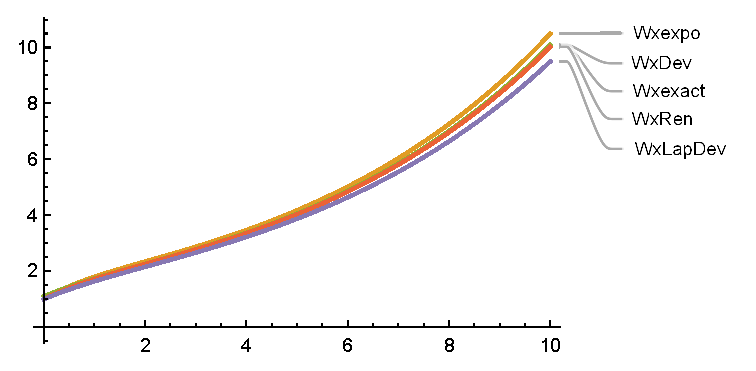
\includegraphics[width=\textwidth]{MixExp83W.eps}
        \caption{$W_q(x)$  (in black)}
        \label{fig:MixExp83W}
    \end{subfigure}
    ~
    \\
    \begin{subfigure}[b]{0.8\textwidth}
        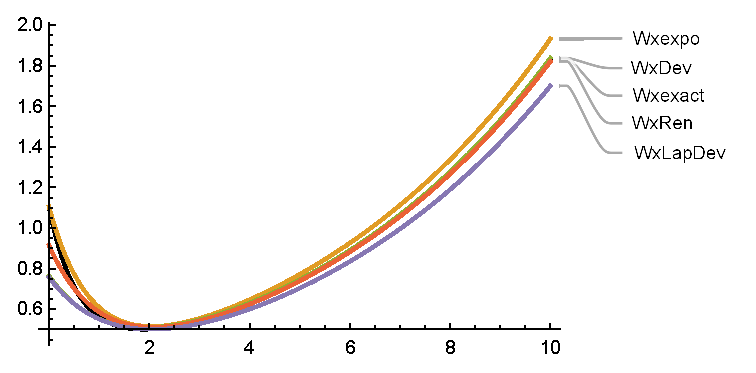
\includegraphics[width=\textwidth]{MixExp83W1}
        \caption{$W'_q(x)$}
        \label{fig:MixExp83W1}
    \end{subfigure}
    ~
    \\
    \begin{subfigure}[b]{0.8\textwidth}
        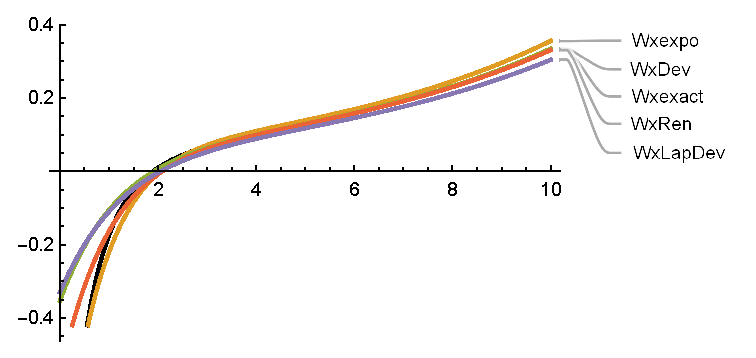
\includegraphics[width=\textwidth]{MixExp83W2}
        \caption{$W''_q(x)$}
        \label{fig:MixExp83W2}
    \end{subfigure}
    \caption{Plots of $W_q(x)$, $W'_q(x)$, and $W''_q(x)$ of the exact solution and the approximations for $f(x)=\frac{12}{83 }e^{-x}+\frac{42}{83} e^{-2 x}+\frac{150}{83}e^{-3x}$, $c=1$, $q=\fr{5}{48}$.}\label{fig:MixExp83}
\end{figure}

Continuing, from the parameters of the process, one can obtain the approximations to the scale function $W_q$ as described in the earlier section. Table \ref{table:MixExp83} gives a summary of the values of $\Phi_q$ and $b_{DeF}$ obtained from these approximations, as well as the relative errors %each one's percent deviation 
from the exact value. \footnote{Percent relative error is computed as the absolute value of the difference between the approximation and the exact, divided by the exact value, times 100. Differences in values when computed from the table and the displayed value may be explained by rounding off errors.}
We can observe a relative error  of less than $2\%$ for each of the approximations' $\Phi_q$ value, with the DeVylder approximation's $\Phi_q$ beating the others. %Considering the optimal barrier $b_{DeF}$ obtained from each, we observe only the DeVylder approximation's $b_{DeF}$ to have a relative error  of less than $7 \%$.

We also tried varying the safety loading factor $\theta$, keeping the density $f$ and the discount rate $q$ to be the same. Over certain values of $\theta \in [0, 263/235]$ we observe the trend of the DeVylder approximation exhibiting the least relative error  in approximating $\Phi_q$. Though the DeVylder approximations displayed increasing errors for decreasing values of $\theta$, the errors never went above $2\%$. A table summarizing the results can be found at table \ref{table:MixExp83Phiq}. Unlike this observation for $\Phi_q$, we are unable to conclude anything when looking at the approximate values for $b_{DeF}$. For $\theta=43/235, 23/235, 3/235$, all of the approximations yielded $b_{DeF}=0$ as the optimal barrier. This turned out to be true for $\theta=3/235$.
\beR {Note (see \fe \cite[Sec. 3]{AGV}) that the necessary, and in our case sufficient condition for the nonnegativity of the optimal dividends barrier is $W_{\q}'' (0_+) <0 \Eq (\frac {\lambda+ \q }  c )^2 < \frac {\lambda}  c f(0)$. Here, this condition is \satd\ for   the exact when $\th \geq ...$. For the approximations, it is \satd\ at ...  }
\eeR

\begin{table}[!h]
\begin{tabular}{|l|l|l|l|l|}
\hline
       & \begin{tabular}[c]{@{}l@{}}Dominant   exponent \\ $\Phi_q$\end{tabular} & \begin{tabular}[c]{@{}l@{}}Percent   relative error\\ ($\Phi_q$)\end{tabular} & \begin{tabular}[c]{@{}l@{}}Optimal barrier\\ $b_{DeF}$\end{tabular} & \begin{tabular}[c]{@{}l@{}}Percent   relative error\\ ($b_{DeF}$)\end{tabular} \\ \hline
Exact  & 0.18198                                                               & 0                                                                           & 1.89732                                                      & 0                                                                       \\ \hline
Expo   & 0.184095                                                              & 1.162215628                                                                 & 2.04608                                                      & 7.840532962                                                             \\ \hline
Dev    & 0.182011                                                              & 0.017034839                                                                 & 1.91233                                                      & 0.79111589                                                              \\ \hline
Renyi  & 0.181708                                                              & 0.149466974                                                                 & 2.08136                                                      & 9.699997892                                                             \\ \hline
LapDev & 0.178939                                                              & 1.671062754                                                                 & 2.04661                                                      & 7.868467101                                                             \\ \hline
\end{tabular}
\caption{Exact and approximate values of $\Phi_q$ and $b_{DeF}$ for $f(x)=\frac{12}{83 }e^{-x}+\frac{42}{83} e^{-2 x}+\frac{150}{83}e^{-3x}$, $c=1$, $q=\fr{5}{48}$. The DeVylder approximation displayed the least relative error  among the four approximations considered.}
\label{table:MixExp83}
\end{table}

\begin{table}[!h]
\begin{tabular}{|l|l|l|l|l|}
\hline
$\theta$ & Closest approximation & $\Phi_q$   exact & $\Phi_q$ approximation & \% error   $\Phi_q$ \\ \hline
263/235    & Dev                   & 0.18198        & 0.182011      & 0.0168217         \\ \hline
243/235    & Dev                   & 0.194712       & 0.194754      & 0.0213671         \\ \hline
223/235    & Dev                   & 0.209221       & 0.209279      & 0.0274827         \\ \hline
203/235    & Dev                   & 0.225876       & 0.225957      & 0.0358309         \\ \hline
183/235    & Dev                   & 0.245146       & 0.245262      & 0.0474032         \\ \hline
163/235    & Dev                   & 0.267635       & 0.267806      & 0.0637063         \\ \hline
143/235    & Dev                   & 0.294126       & 0.294382      & 0.0870647         \\ \hline
123/235    & Dev                   & 0.325643       & 0.326038      & 0.121115          \\ \hline
103/235    & Dev                   & 0.363539       & 0.364163      & 0.171618          \\ \hline
83/235     & Dev                   & 0.40961        & 0.410625      & 0.247788          \\ \hline
63/235     & Dev                   & 0.466261       & 0.46796       & 0.364457          \\ \hline
43/235     & Dev                   & 0.536719       & 0.539647      & 0.545532          \\ \hline
23/235     & Dev                   & 0.62533        & 0.630516      & 0.829419          \\ \hline
3/235      & Dev                   & 0.737962       & 0.747389      & 1.27736           \\ \hline
\end{tabular}
\caption{Exact and approximate values of $\Phi_q$ for $f(x)=\frac{12}{83 }e^{-x}+\frac{42}{83} e^{-2 x}+\frac{150}{83}e^{-3x}$, varying the value of $\theta$. The DeVylder approximation displayed the least relative error  among the four approximations considered.}
\label{table:MixExp83Phiq}
\end{table}

\begin{table}[!h]
\begin{tabular}{|l|l|l|l|l|}
\hline
$\theta$ & Closest approximation & Barrier exact & Barrier approx & \% error Barrier \\ \hline
263/235 & Dev    & 1.89732   & 1.91233  & 0.791183 \\ \hline
243/235 & Dev    & 1.79954   & 1.78002  & 1.08482  \\ \hline
223/235 & LapDev & 1.69334   & 1.74547  & 3.07875  \\ \hline
203/235 & LapDev & 1.57785   & 1.56951  & 0.528553 \\ \hline
183/235 & Ren    & 1.45224   & 1.52484  & 4.9989   \\ \hline
163/235 & Ren    & 1.31579   & 1.33691  & 1.60463  \\ \hline
143/235 & Ren    & 1.16804   & 1.12368  & 3.79796  \\ \hline
123/235 & Expo   & 1.00898   & 1.04123  & 3.19653  \\ \hline
103/235 & Expo   & 0.839228  & 0.794964 & 5.27444  \\ \hline
83/235  & Expo   & 0.660338  & 0.513179 & 22.2854  \\ \hline
63/235  & Expo   & 0.474896  & 0.196234 & 58.6785  \\ \hline
43/235  & Expo   & 0.286563  & 0        & 100      \\ \hline
23/235  & Expo   & 0.0998863 & 0        & 100      \\ \hline
3/235   & Exact  & 0         & 0        & 0        \\ \hline
\end{tabular}
\caption{Exact and approximate values of $b_{DeF}$ for $f(x)=\frac{12}{83 }e^{-x}+\frac{42}{83} e^{-2 x}+\frac{150}{83}e^{-3x}$, varying the value of $\theta$. No single approximation displayed a noticeable advantage over the others.}
\label{table:MixExp83Bar}
\end{table} 
%\vfil \eject

%\newpage



\subsection{A Cram\'{e}r-Lundberg process with non-hyperexponential claims of order 5} \label{e:NH5mm}
Consider the Cram\'{e}r-Lundberg process with density of claims $$f(x)=\frac{5}{2 }e^{-5x}+\frac{4}{5} e^{-4 x}-\frac{1}{5}e^{-3x}- \frac{1}{5}e^{-2x}+ \frac{1}{20}e^{-x}$$
and $c=\frac{23}{90}$, $\l=\frac{7}{12}$, $\th= 1$, $p=23/180$, $\rho = \frac{1}{2}$, $q=\frac{1}{10}$.

The Laplace exponent of this process is $ \kappa(s) = \frac{23 s}{90} -\frac{s}{20 (s+1)}+\frac{s}{10 (s+2)}+\frac{s}{15 (s+3)}-\frac{s}{5 (s+4)}-\frac{s}{2 (s+5)}$ and from here the scale function is
\bea
W_q(x) & = -0.0831561\  e^{(-4.35135 x)} + 0.684818\  e^{(-2.65126 x)} - 0.595164\ e^{(-0.837877 x)} + 6.02604\  e^{(0.666084 x)} \\ & - 2.11949\  e^{(-2.57585 x)} \cos[0.811233 x]  + 2.39748 \  e^{(-2.57585 x)} \sin[0.811233 x]
\eea

\begin{figure}[!h]
    \centering
    \begin{subfigure}[b]{0.8\textwidth}
        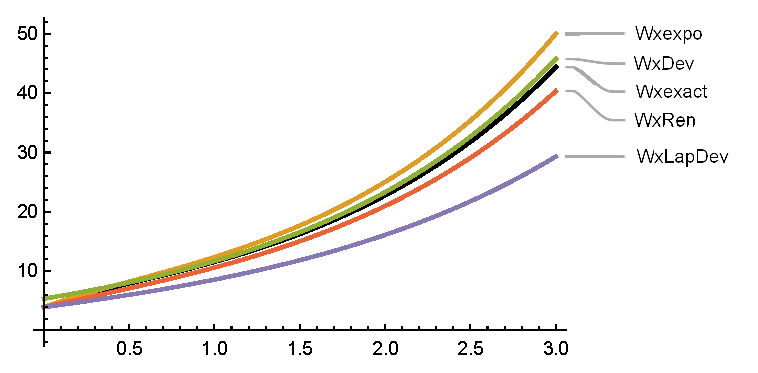
\includegraphics[width=\textwidth]{NH5mmW}
        \caption{$W_q(x)$ (in black)}
        \label{fig:NH5mmW}
    \end{subfigure}
    ~
    \\
    \begin{subfigure}[b]{0.8\textwidth}
        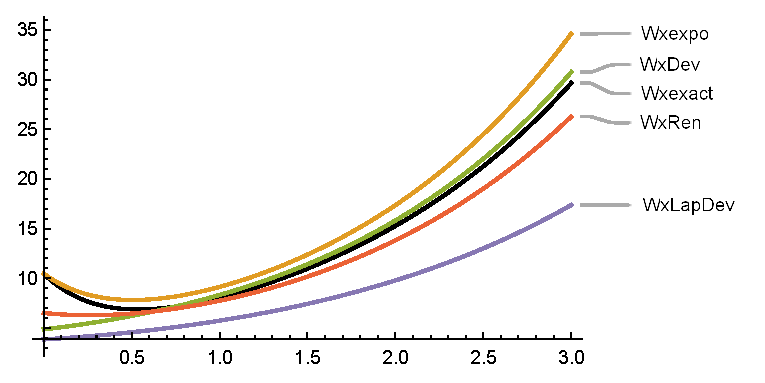
\includegraphics[width=\textwidth]{NH5mmW1}
        \caption{$W'_q(x) $}
        \label{fig:NH5mmW1}
    \end{subfigure}
    ~
    \\
    \begin{subfigure}[b]{0.8\textwidth}
        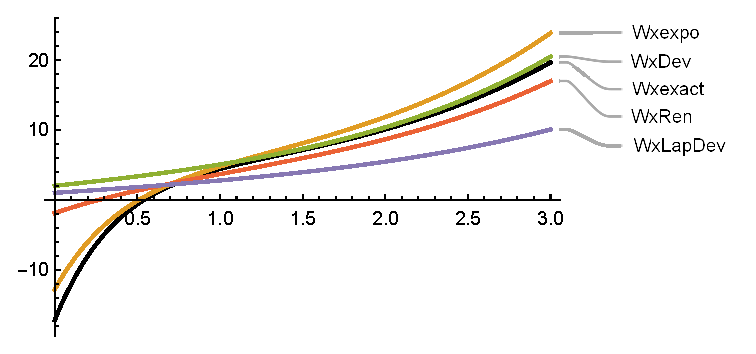
\includegraphics[width=\textwidth]{NH5mmW2}
        \caption{$W''_q(x)$}
        \label{fig:NH5mmW2}
    \end{subfigure}
    \caption{Plots of $W_q(x)$, $W'_q(x)$, and $W''_q(x)$ of the exact solution and the approximations, for $f(x)=\frac{5}{2 }e^{-5x}+\frac{4}{5} e^{-4 x}-\frac{1}{5}e^{-3x}- \frac{1}{5}e^{-2x}+ \frac{1}{20}e^{-x}$, $\theta=1$, $q=1/10$}
    \label{fig:NH5mm}
\end{figure}


As seen in table \ref{table:NH5mm}, the approximations for  $W_q$ give again the DeVylder as the closest approximation when looking at the $\Phi_q$ value. However, $W'_q$ for the DeVylder attains its minimum at $x=0$, which is relatively far from the exact barrier at $b_{DeF}=0.538$. The exponential approximation shows the best barrier approximate at $x=0.506947$.

The lack of a minimum of $W'_q$ for the DeVylder and the Laplace DeVylder approximations inside the interval $x \in (0,3)$ can be seen clearly in the plots in figure \ref{fig:NH5mmW1}. The lack of zero of the corresponding $W''_q$ plots in figure \ref{fig:NH5mmW2} supports this idea. The exponential approximation has the closest root to the exact at around $x=0.5$.

\begin{table}[!h]
\begin{tabular}{|l|l|l|l|l|}
\hline
       & \begin{tabular}[c]{@{}l@{}}Dominant   exponent \\ $\Phi_q$\end{tabular} & \begin{tabular}[c]{@{}l@{}}Percent   relative error\\ ($\Phi_q$)\end{tabular} & \begin{tabular}[c]{@{}l@{}}Optimal barrier\\ $b_{DeF}$\end{tabular} & \begin{tabular}[c]{@{}l@{}}Percent   relative error\\ ($b_{DeF}$)\end{tabular} \\ \hline
Exact  & 0.666084 & 0        & 0.538    & 0       \\ \hline
Expo   & 0.691616 & 3.8331   & 0.506947 & 5.77181 \\ \hline
Dev    & 0.670061 & 0.596931 & 0        & 100     \\ \hline
Renyi  & 0.650448 & 2.34749  & 0.260532 & 51.5739 \\ \hline
LapDev & 0.587976 & 11.7265  & 0        & 100     \\ \hline
\end{tabular}
\caption{Exact and approximate values of $\Phi_q$ and $b_{DeF}$ for $f(x)=\frac{5}{2 }e^{-5x}+\frac{4}{5} e^{-4 x}-\frac{1}{5}e^{-3x}- \frac{1}{5}e^{-2x}+ \frac{1}{20}e^{-x}$, $\theta=1$, $q=1/10$. The DeVylder approximation displayed the least percent relative error in approximating $\Phi_q$, but struggled in approximating $b_{DeF}$.}
\label{table:NH5mm}
\end{table}


\begin{table}[!h]
\begin{tabular}{|l|l|l|l|l|}
\hline
$\theta$ & Closest approximation & $\Phi_q$   exact & $\Phi_q$ approximation & \% error   $\Phi_q$ \\ \hline
1   & Dev                     & 0.666084       & 0.670061 & 0.596931          \\ \hline
0.9 & Dev                     & 0.721302       & 0.726797 & 0.761704          \\ \hline
0.8 & Dev                     & 0.785584       & 0.793322 & 0.985015          \\ \hline
0.7 & Dev                     & 0.861148       & 0.872279 & 1.29261           \\ \hline
0.6 & Dev                     & 0.950932       & 0.967325 & 1.72389           \\ \hline
0.5 & Dev                     & 1.05887        & 1.08366  & 2.34057           \\ \hline
0.4 & Dev                     & 1.19032        & 1.22891  & 3.24173           \\ \hline
0.3 & Dev                     & 1.35264        & 1.41474  & 4.59125           \\ \hline
0.2 & Dev                     & 1.55609        & 1.65988  & 6.6701            \\ \hline
0.1 & Expo                    & 1.81514        & 1.95652  & 7.78877           \\ \hline
\end{tabular}
\caption{Exact and approximate values of $\Phi_q$ for $f(x)=\frac{5}{2 }e^{-5x}+\frac{4}{5} e^{-4 x}-\frac{1}{5}e^{-3x}- \frac{1}{5}e^{-2x}+ \frac{1}{20}e^{-x}$, varying the value of $\theta$. The DeVylder approximation displayed the least percent relative error among the four approximations considered.}
\label{table:NH5mmPhiq}
\end{table}


\begin{table}[]
\begin{tabular}{|l|l|l|l|l|}
\hline
$\theta$ & Closest approximation & Barrier exact & Barrier approx & \% error Barrier \\ \hline
1   & Expo                    & 0.538           & 0.506947  & 5.77181            \\ \hline
0.9 & Expo                    & 0.496513        & 0.448391  & 9.69186            \\ \hline
0.8 & Expo                    & 0.448937        & 0.382485  & 14.8021            \\ \hline
0.7 & Expo                    & 0.394055        & 0.308318  & 21.7575            \\ \hline
0.6 & Expo                    & 0.330415        & 0.225085  & 31.8783            \\ \hline
0.5 & Expo                    & 0.256331        & 0.13227   & 48.3988            \\ \hline
0.4 & Expo                    & 0.169933        & 0.0299613 & 82.3687            \\ \hline
0.3 & Expo                    & 0.0693293       & 0         & 100                \\ \hline
0.2 & Exact                   & 0               & 0         & 0                  \\ \hline
0.1 & Exact                   & 0               & 0         & 0                  \\ \hline
\end{tabular}
\caption{Exact and approximate values of $\Phi_q$ for $f(x)=\frac{5}{2 }e^{-5x}+\frac{4}{5} e^{-4 x}-\frac{1}{5}e^{-3x}- \frac{1}{5}e^{-2x}+ \frac{1}{20}e^{-x}$, varying the value of $\theta$. The exponential approximation displayed the least percent relative error among the four approximations considered.}
\label{table:NH5mmBar}
\end{table} 
\newpage

\subsection{A Cram\'{e}r-Lundberg process with a matrix exponential density} \label{e:MatExp6220}

Next we consider an example produced by taking a Cram\'{e}r-Lundberg process with matrix exponential density of claims $f(x)=\a e^{A x} (-A) \bff 1 $, where $\a=(-2.4, 0.9 , 2.5),  A = \bep
   {-6.2, 2, 0}\\
   {2, -9, 1}\\
   {1, 0, -3}\eep$
and $\l=1$, $\th=1$, $q=\fr{1}{10}$.

The Laplace exponent of this process is
$\kappa(s) = 1.3249 s -\frac{3.34053 s}{s+2.87761}+\frac{3.03143 s}{s+5.34047}-\frac{0.690902 s}{s+9.98192}$ and the scale function is
\bea
W_q(x)  &= -0.0655864 e^{-9.35143 x}+0.149742 e^{-6.89805 x}-0.676982 e^{-1.26245 x}+1.3476 e^{0.142175 x}.
\eea

\begin{figure}[!h]
    \centering
    \begin{subfigure}[b]{0.8\textwidth}
        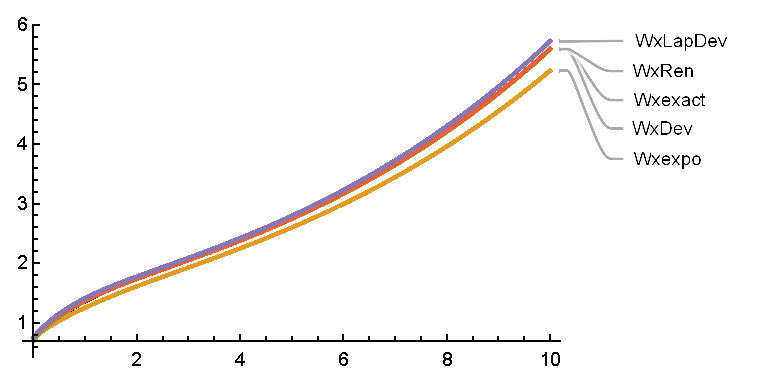
\includegraphics[width=\textwidth]{MatExp6220W}
        \caption{$W_q(x)$  (in black)}
        \label{fig:MatExp6220W}
    \end{subfigure}
    ~
    \\
    \begin{subfigure}[b]{0.8\textwidth}
        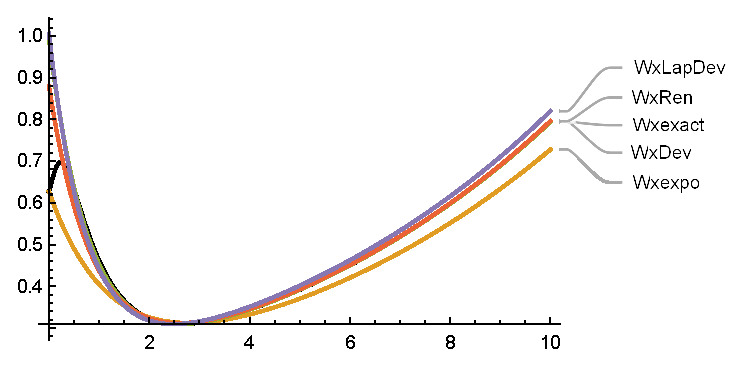
\includegraphics[width=\textwidth]{MatExp6220W1}
        \caption{$W'_q(x)$}
        \label{fig:MatExp6220W1}
    \end{subfigure}
    ~
    \\
    \begin{subfigure}[b]{0.8\textwidth}
        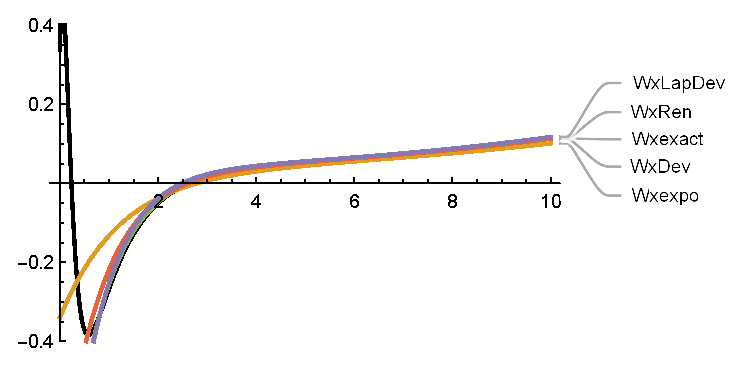
\includegraphics[width=\textwidth]{MatExp6220W2}
        \caption{$W''_q(x)$}
        \label{fig:MatExp6220W2}
    \end{subfigure}
    \caption{Plots of $W_q(x)$, $W'_q(x)$, and $W''_q(x)$ of the exact solution and the approximations for $f(x)=\a e^{A x} (-A) \bff 1 $, $\th=1$, $q=\fr{1}{10}$.}\label{fig:MatExp6220}
\end{figure}


\begin{table}[!h]
\begin{tabular}{|l|l|l|l|l|}
\hline
       & \begin{tabular}[c]{@{}l@{}}Dominant   exponent \\ $\Phi_q$\end{tabular} & \begin{tabular}[c]{@{}l@{}}Percent   relative error\\ ($\Phi_q$)\end{tabular} & \begin{tabular}[c]{@{}l@{}}Optimal barrier\\ $b_{DeF}$\end{tabular} & \begin{tabular}[c]{@{}l@{}}Percent   relative error\\ ($b_{DeF}$)\end{tabular} \\ \hline
Exact  & 0.142175                   & 0                                 & 2.61925              & 0                             \\ \hline
Expo   & 0.139202                   & 2.09118                           & 2.79162              & 6.58074                       \\ \hline
Dev    & 0.142174                   & 0.00104491                        & 2.60329              & 0.609153                      \\ \hline
Renyi  & 0.142238                   & 0.0439717                         & 2.59638              & 0.873044                      \\ \hline
LapDev & 0.143232                   & 0.743272                          & 2.48327              & 5.19155                       \\ \hline
\end{tabular}
\caption{Exact and approximate values of $\Phi_q$ and $b_{DeF}$ for $f(x)=\a e^{A x} (-A) \bff 1 $, $\th=1$, $q=\fr{1}{10}$. The DeVylder approximation displayed the least percent relative error among the four approximations considered.}
\label{table:MatExp6220}
\end{table}


\begin{table}[!h]
\begin{tabular}{|l|l|l|l|l|}
\hline
$\theta$ & Closest approximation & $\Phi_q$   exact & $\Phi_q$ approximation & \% error   $\Phi_q$ \\ \hline
1   & Dev                     & 0.142175       & 0.142174 & 0.00104491        \\ \hline
0.9 & Dev                     & 0.156039       & 0.156036 & 0.00148235        \\ \hline
0.8 & Dev                     & 0.172688       & 0.172684 & 0.00216274        \\ \hline
0.7 & Dev                     & 0.192979       & 0.192973 & 0.00325715        \\ \hline
0.6 & Dev                     & 0.218117       & 0.218106 & 0.0050835         \\ \hline
0.5 & Dev                     & 0.249825       & 0.249804 & 0.0082542         \\ \hline
0.4 & Dev                     & 0.290594       & 0.290553 & 0.013988          \\ \hline
0.3 & Dev                     & 0.344047       & 0.343962 & 0.0247701         \\ \hline
0.2 & Dev                     & 0.415404       & 0.415214 & 0.0457098         \\ \hline
0.1 & Dev                     & 0.512          & 0.511554 & 0.0871333         \\ \hline
\end{tabular}
\caption{Exact and approximate values of $\Phi_q$ for $f(x)=\a e^{A x} (-A) \bff 1 $, varying the value of $\theta$. The DeVylder approximation displayed the least percent relative error among the four approximations considered.}
\label{table:MatExp6220Phiq}
\end{table}



\begin{table}[!h]
\begin{tabular}{|l|l|l|l|l|}
\hline
$\theta$ & Closest approximation & Barrier exact & Barrier approx & \% error Barrier \\ \hline
1   & Dev                     & 2.61925         & 2.60329  & 0.609154           \\ \hline
0.9 & Dev                     & 2.52243         & 2.50437  & 0.716072           \\ \hline
0.8 & Expo                    & 2.39997         & 2.39528  & 0.195427           \\ \hline
0.7 & Dev                     & 2.24344         & 2.22233  & 0.941111           \\ \hline
0.6 & Dev                     & 2.04159         & 2.01986  & 1.06465            \\ \hline
0.5 & Dev                     & 1.77996         & 1.75855  & 1.20296            \\ \hline
0.4 & Dev                     & 0               & 1.4216   & -                  \\ \hline
0.3 & Expo                    & 0               & 0.518511 & -                  \\ \hline
0.2 & Exact                   & 0               & 0        & -                  \\ \hline
0.1 & Exact                   & 0               & 0        & -                  \\ \hline
\end{tabular}
\caption{Exact and approximate values of $b_{DeF}$ for $f(x)=\a e^{A x} (-A) \bff 1 $, varying the value of $\theta$.  The DeVylder approximation displayed the least percent relative error among the four approximations considered.}
\label{table:MatExp6220Bar}
\end{table}
\newpage

\subsection{A Cram\'{e}r-Lundberg process with an Erlang density} \label{e:AzcueM}

In the following example, we study a \CL\ model with  $Erlang(2,1)$  density of claims $f(x) = 10 \le(x e^{-x}\ri)$ and  $\l=10, \th = \frac{7}{100},\  c = \frac{107}{5},\ q=\frac{1}{10}.$

The Laplace exponent of this process is
$\kappa(s) = 21.4 s -\frac{10 s}{s+1}-\frac{10 s}{(s+1)^2}$ and the scale function is
\bea
W_q(x)  &= 0.00517511 e^{-1.48825 x}-0.23639 e^{-0.0793553 x}+0.277943 e^{0.0395672 x}.
\eea

\begin{figure}[!h]
    \centering
    \begin{subfigure}[b]{0.8\textwidth}
        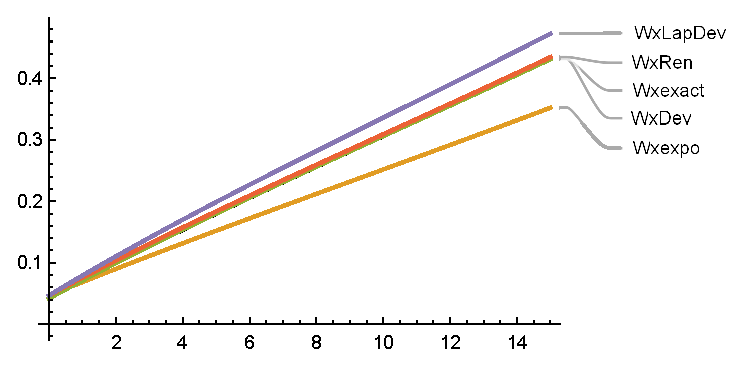
\includegraphics[width=\textwidth]{AzcueMW}
        \caption{$W_q(x)$  (in black)}
        \label{fig:AzcueMW}
    \end{subfigure}
    ~
    \\
    \begin{subfigure}[b]{0.8\textwidth}
        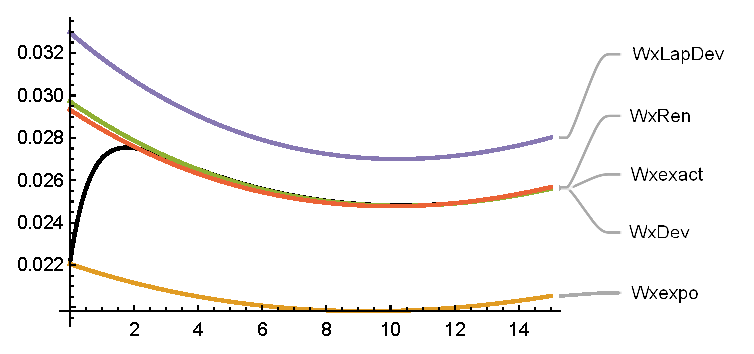
\includegraphics[width=\textwidth]{AzcueMW1}
        \caption{$W'_q(x)$}
        \label{fig:AzcueMW1}
    \end{subfigure}
    ~
    \\
    \begin{subfigure}[b]{0.8\textwidth}
        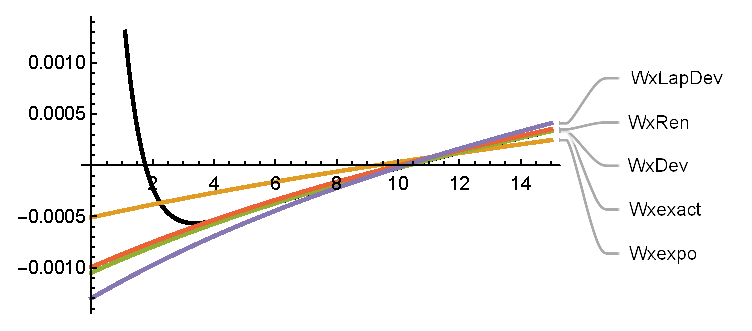
\includegraphics[width=\textwidth]{AzcueMW2}
        \caption{$W''_q(x)$}
        \label{fig:AzcueMW2}
    \end{subfigure}
    \caption{Plots of $W_q(x)$, $W'_q(x)$, and $W''_q(x)$ of the exact solution and the approximations for $f(x) = 10 \le(x e^{-x}\ri)$, $\th = \frac{7}{100}$, $q=\fr{1}{10}$.}\label{fig:AzcueM}
\end{figure}


\begin{table}[!h]
\begin{tabular}{|l|l|l|l|l|}
\hline
       & \begin{tabular}[c]{@{}l@{}}Dominant   exponent \\ $\Phi_q$\end{tabular} & \begin{tabular}[c]{@{}l@{}}Percent   relative error\\ ($\Phi_q$)\end{tabular} & \begin{tabular}[c]{@{}l@{}}Optimal barrier\\ $b_{DeF}$\end{tabular} & \begin{tabular}[c]{@{}l@{}}Percent   relative error\\ ($b_{DeF}$)\end{tabular} \\ \hline
Exact  & 0.142175                   & 0                                 & 2.61925              & 0                             \\ \hline
Expo   & 0.139202                   & 2.09118                           & 2.79162              & 6.58074                       \\ \hline
Dev    & 0.142174                   & 0.00104491                        & 2.60329              & 0.609153                      \\ \hline
Renyi  & 0.142238                   & 0.0439717                         & 2.59638              & 0.873044                      \\ \hline
LapDev & 0.143232                   & 0.743272                          & 2.48327              & 5.19155                       \\ \hline
\end{tabular}
\caption{Exact and approximate values of $\Phi_q$ and $b_{DeF}$ for $f(x) = 10 \le(x e^{-x}\ri)$, $\th = \frac{7}{100}$, $q=\fr{1}{10}$. The DeVylder approximation displayed the least percent relative error among the four approximations considered.}
\label{table:AzcueM}
\end{table}
\newpage

\subsection{A Cram\'{e}r-Lundberg process with a matrix exponential density} \label{e:MatExpCos}

In the following example, we study a \CL\ model with density of claims given by
\begin{align*}
f(x)=& u e^{-a x} 2 \cos ^{2}\left(\frac{\omega x+\phi}{2}\right)=u e^{-a x}(1+\cos (\omega x+\phi))=\\=& e^{-a x}(u+u \cos (\phi) \cos (\omega x)-u \sin (\phi) \sin (\omega x))
\end{align*}
where
\[u=\frac{a\left(a^{2}+\omega^{2}\right)}{a^{2}+\omega^{2}+a^{2} \cos (\phi)-a \omega \sin (\phi)}. \]
One can check that $\int f(x) d x=1$ with such value of $u$.

Assuming further that $a=1$, $\phi=2$, $\omega=20$, and that $\theta=1$, $q=1/10$, the Laplace exponent for this process is
$\kappa(s) = \frac{s \left(2.09898 s^3+5.29695 s^2+843.502 s+420.846\right)}{(s+1.) \left(s^2+2. s+401.\right)}$ and the scale function is
\begin{align*}
W_q(x)  &= 0.824723 e^{0.0881484 x} -0.348141 e^{-0.540677 x} \\
   &+e^{-1.0117 x} \cos (19.9957 x) ~\Big( -(0.000285494\, +0.0000804151 i) \sin (39.9914 x)\\
   &-(0.0000804151\, +0.000285494 i)+(-0.0000804151+0.000285494 i) \cos (39.9914 x) \Big)\\
   &+e^{-1.0117 x} \sin (19.9957 x) ~\Big( -(0.0000804151\, -0.000285494 i) \sin (39.9914 x) \\
   & +(0.000285494\, +0.0000804151 i) \cos (39.9914 x)-(0.000285494\, -0.0000804151 i) \Big).
\end{align*}

\begin{figure}[!h]
    \centering
    \begin{subfigure}[b]{0.8\textwidth}
        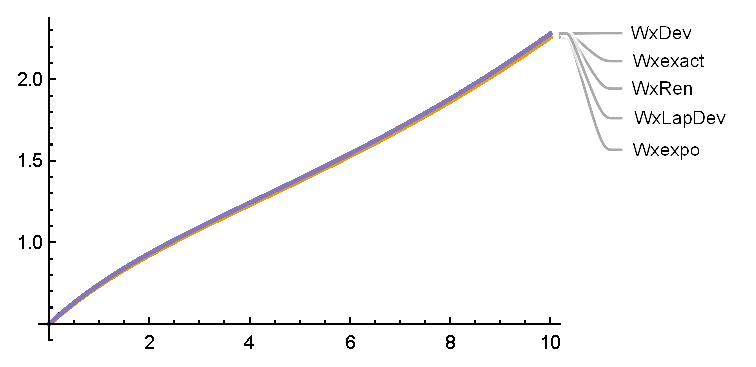
\includegraphics[width=\textwidth]{MatExpCosW}
        \caption{$W_q(x)$  (in black)}
        \label{fig:MatExpCosW}
    \end{subfigure}
    ~
    \\
    \begin{subfigure}[b]{0.8\textwidth}
        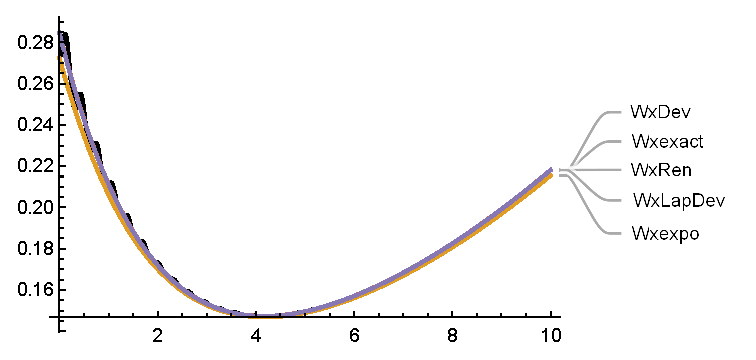
\includegraphics[width=\textwidth]{MatExpCosW1}
        \caption{$W'_q(x)$}
        \label{fig:MatExpCosW1}
    \end{subfigure}
    ~
    \\
    \begin{subfigure}[b]{0.8\textwidth}
        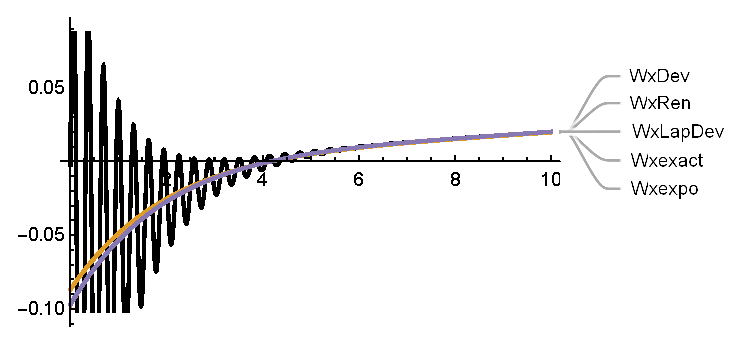
\includegraphics[width=\textwidth]{MatExpCosW2}
        \caption{$W''_q(x)$}
        \label{fig:MatExpCosW2}
    \end{subfigure}
    \caption{Plots of $W_q(x)$, $W'_q(x)$, and $W''_q(x)$ of the exact solution and the approximations for $f(x)= u e^{-a x} 2 \cos ^{2}\left(\frac{\omega x+\phi}{2}\right)$, $\th =1$, $q=\fr{1}{10}$.}\label{fig:MatExpCos}
\end{figure}


\begin{table}[!h]
\begin{tabular}{|l|l|l|l|l|}
\hline
       & \begin{tabular}[c]{@{}l@{}}Dominant   exponent \\ $\Phi_q$\end{tabular} & \begin{tabular}[c]{@{}l@{}}Percent   relative error\\ ($\Phi_q$)\end{tabular} & \begin{tabular}[c]{@{}l@{}}Optimal barrier\\ $b_{DeF}$\end{tabular} & \begin{tabular}[c]{@{}l@{}}Percent   relative error\\ ($b_{DeF}$)\end{tabular} \\ \hline
Exact  & 0.0881484                  & 0                                 & 4.38201              & 0                             \\ \hline
Expo   & 0.0878658                  & 0.32053                           & 4.42263              & 0.927122                      \\ \hline
Dev    & 0.0881484                  & 6.11743*10\textasciicircum{}-6    & 4.39745              & 0.352331                      \\ \hline
Renyi  & 0.0881481                  & 0.000314617                       & 4.39788              & 0.362284                      \\ \hline
LapDev & 0.0881449                  & 0.00395543                        & 4.3982               & 0.369586                      \\ \hline
\end{tabular}
\caption{Exact and approximate values of $\Phi_q$ and $b_{DeF}$ for $f(x)= u e^{-a x} 2 \cos ^{2}\left(\frac{\omega x+\phi}{2}\right)$, $\th =1$, $q=\fr{1}{10}$. The DeVylder approximation displayed the least percent relative error among the four approximations considered.}
\label{table:MatExpCos}
\end{table}

%\section{Examples of scale computations for \CL \ models \la{ex:1}}

In this section, examples along with numerical simulations will be presented. Starting with the case of a \CL\ model with exponential mixtures jumps of order three, we plot the graphs \re{of $W_q$, and also of $W'_q$, $W''_q$, when they exhibit oscillations, and determine the "winning approximation".}

\re{\Ito the best approximation is ...}

In the \textit{example \eqr{NH5}}, we try to see what happens in the case of order five of a non-hyperexponential jump density. Finally drawing upon the BUtools package, we deal with a \CL\ model with a non phase-type jump density.\re{was  that checked?}


\beXa
Consider a Cram\'{e}r-Lundberg process with density function
$\frac{150}{83} e^{-3 x}+ \frac{42}{83} e^{-2 x} + \frac{12 }{83} e^{-x}$, and $c=1$,  $\l=\frac{83}{48}$, $\th=\fr{263}{235}$, $q=\fr{5}{48}$, $p= \fr{263}{498}$.
The Laplace exponent of this process is
$\kappa(s) = s - \frac{12 s}{83 (s+1)}-\frac{21 s}{83 (s+2)}-\frac{50 s}{83 (s+3)}$ and from this one can (numerically) invert $\frac{1}{\kappa(s) - q} =  \H{W}_q(s)$ to obtain the scale function

\iffalse
\fn[4]{This was produced by taking
$\Fq=\frac{1}{3}, c=1$ and
a negative Wiener-Hopf factor
$$\f_-(s)=\frac{\left(\frac{s}{3}+1\right) \left(\frac{s}{2}+1\right) (s+1)}{\left(\frac{2 s}{5}+1\right) \left(\frac{2 s}{3}+1\right) (2
   s+1)}$$
   with poles $-\fr 1 2, -\fr 3 2, -\fr 5 2$.}
\fi

\bea
W_q(x)  &= -0.0813294 e^{(-2.60997 x)} - 0.179472 e^{(-1.68854 x)} \\ &- 0.373887 e^{(-0.779311 x)}  + 1.63469 e^{(0.18198 x)}.
\eea


From here one can obtain the dominant exponent $\Phi_q = 0.18198$, and since the minimum of $W_q'$ is at $b^*=1.89732$, we conclude that this is the optimal barrier that would maximize dividends.

Continuing, from the parameters of the process, one can obtain the approximations to the scale function $W_q$ as described in the earlier section. Table \ref{table:sample1} gives a summary of the values of $\Phi_q$ and $b^*$ obtained from these approximations, as well as the each one's percent deviation from the exact value. Figure \ref{fig:sample1} shows the plots of $W_q$ as well as its first two derivatives.

From table \ref{table:sample1}, we can observe a percent relative error of less than $2\%$ for each of the approximations' $\Phi_q$ value, with the DeVylder approximation's $\Phi_q$ beating the others. Considering the optimal barrier $b^*$ obtained from each, we observe only the DeVylder approximation's $b^*$ to have a percent relative error of less than $7 \%$.


\begin{table} 
\begin{tabular}{|l|l|l|l|l|} 
\hline
       & \begin{tabular}[c]{@{}l@{}}Dominant   exponent \\ $\Phi_q$\end{tabular} & \begin{tabular}[c]{@{}l@{}}Percent   relative error\\ ($\Phi_q$)\end{tabular} & \begin{tabular}[c]{@{}l@{}}Optimal barrier\\ $b^*$\end{tabular} & \begin{tabular}[c]{@{}l@{}}Percent   relative error\\ ($b^*$)\end{tabular} \\ \hline
Exact  & 0.18198                                                               & 0                                                                           & 1.89732                                                      & 0                                                                       \\ \hline
Expo   & 0.184095                                                              & 1.162215628                                                                 & 2.04608                                                      & 7.840532962                                                             \\ \hline
Dev    & 0.182011                                                              & 0.017034839                                                                 & 1.91233                                                      & 0.79111589                                                              \\ \hline
Renyi  & 0.181708                                                              & 0.149466974                                                                 & 2.08136                                                      & 9.699997892                                                             \\ \hline
LapDev & 0.178939                                                              & 1.671062754                                                                 & 2.04661                                                      & 7.868467101                                                             \\ \hline
\end{tabular}
\caption{Example 1: Values of $\Phi_q$ and $b^*$ obtained from the approximations and percent relative error when compared to the exact value}
\label{table:sample1}
\end{table}


\begin{figure}
    \centering
    \begin{subfigure}[b]{0.4\textwidth}
        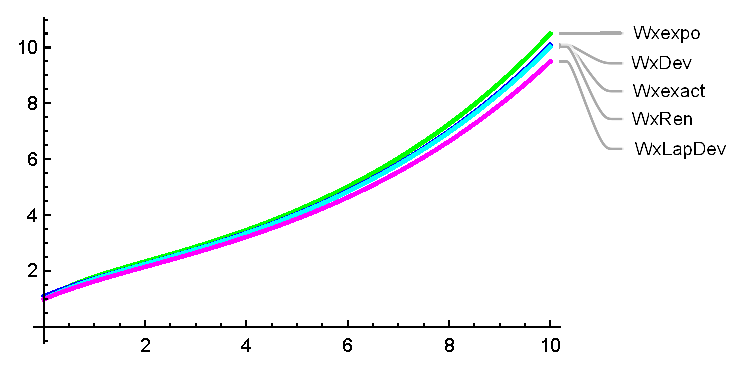
\includegraphics[width=\textwidth]{Wsample1}
        \caption{$W_q(x)$}
        \label{fig:Wsample1}
    \end{subfigure}
    ~ %add desired spacing between images, e. g. ~, \quad, \qquad, \hfill etc. 
      %(or a blank line to force the subfigure onto a new line)
    \begin{subfigure}[b]{0.4\textwidth}
        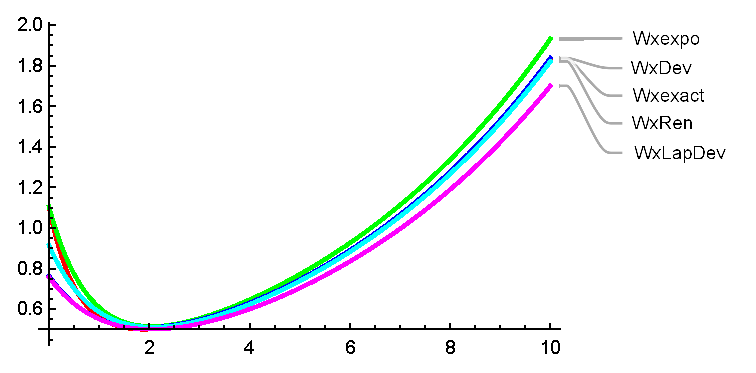
\includegraphics[width=\textwidth]{W1sample1}
        \caption{$W'_q(x)$}
        \label{fig:W1sample1}
    \end{subfigure}
    ~ %add desired spacing between images, e. g. ~, \quad, \qquad, \hfill etc. 
    %(or a blank line to force the subfigure onto a new line)
    \\
    \begin{subfigure}[b]{0.9\textwidth}
        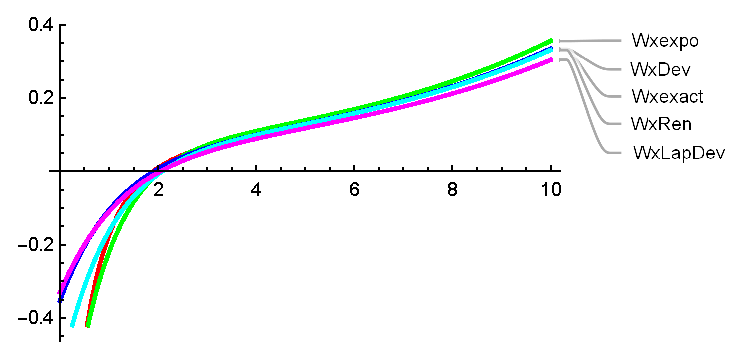
\includegraphics[width=\textwidth]{W2sample1}
        \caption{$W''_q(x)$}
        \label{fig:W2sample1}
    \end{subfigure}
    \caption{Example 1: Plots of $W_q(x)$, $W'_q(x)$, and $W''_q(x)$ of the exact solution and the approximations}\label{fig:sample1}
\end{figure}



\iffalse

The approximation for the \rp\ was already given in Figure \ref{f:MEp1}. The dominant exponents of Renyi and de Vylder are $0.174908, 0.175181$, very close, but a bit smaller than the real $\Fq=0.18198$.

\figu{Wa}{The  Renyi approximation and classic  DeVylder are practically indistinguishable for large $x$
of the exact formula of $W_q(x)$, for $f(x)=\frac{12}{83 }e^{-x}+\frac{42}{83} e^{-2 x}+\frac{150}{83}e^{-3x}$. The   DeVylder-Laplace is rather poor, and so is the naive approximation; overfitting at $0$ seems a bad idea.}{.3}

In  figure \ref{f:Wa}, we draw the exact \sf\ $W_q(x)$, together with the \deV-type and
Renyi    approximations. The figure suggests that the  \re{Renyi \app\ is a lower bound, and that the classic de-Vylder approximation is  the best}. This is investigated in further examples the next section.

As seen in  figure \ref{f:?}   the exact optimal barrier is $b^*=0.866289$, and the Renyi and \re{classic de-Vylder} optimal barriers are \re{$b_R= 0.656067$, ...} 
\fi

\eeXa


\beXa \la{NH5}
Consider the Cram\'{e}r-Lundberg process with density of claims $f(x)=\frac{5}{2 }e^{-5x}+\frac{4}{5} e^{-4 x}-\frac{1}{5}e^{-3x}- \frac{1}{5}e^{-2x}+ \frac{1}{20}e^{-x}$
and $c=\frac{23}{90}$,   $q=\frac{1}{10}$.

One can solve for the other parameters of the process yielding $\l=\frac{7}{12}$, $\th= 1$, $p=23/180$, $\rho = \frac{1}{2}$. The Laplace exponent of this process is $ \kappa(s) = \frac{23 s}{90} -\frac{s}{20 (s+1)}+\frac{s}{10 (s+2)}+\frac{s}{15 (s+3)}-\frac{s}{5 (s+4)}-\frac{s}{2 (s+5)}$ and from here the scale function is
\bea
W_q(x) & = -0.0831561\  e^{(-4.35135 x)} + 0.684818\  e^{(-2.65126 x)} - 0.595164\ e^{(-0.837877 x)} + 6.02604\  e^{(0.666084 x)} \\ & - 2.11949\  e^{(-2.57585 x)} \cos[0.811233 x]  + 2.39748 \  e^{(-2.57585 x)} \sin[0.811233 x]
\eea

\begin{table}[]
\begin{tabular}{|l|l|l|l|l|}
\hline
       & \begin{tabular}[c]{@{}l@{}}Dominant   exponent \\ Phi\_q\end{tabular} & \begin{tabular}[c]{@{}l@{}}Percent   relative error\\ (Phi\_q)\end{tabular} & \begin{tabular}[c]{@{}l@{}}Optimal barrier\\ b*\end{tabular} & \begin{tabular}[c]{@{}l@{}}Percent   relative error\\ (b*)\end{tabular} \\ \hline
Exact  & 0.666084                                                              & 0                                                                           & 0.538                                                        & 0                                                                       \\ \hline
Expo   & 0.691616                                                              & 3.833150173                                                                 & 0.506947                                                     & 5.771933086                                                             \\ \hline
Dev    & 0.670061                                                              & 0.597071841                                                                 & 0.834488                                                     & 55.10929368                                                             \\ \hline
Renyi  & 0.650448                                                              & 2.347451673                                                                 & 0.260532                                                     & 51.5739777                                                              \\ \hline
LapDev & 0.587976                                                              & 11.72644892                                                                 & 0.655954                                                     & 21.92453532                                                             \\ \hline
\end{tabular}
\caption{Example 2: Values of $\Phi_q$ and $b^*$ obtained from the approximations and percent relative error when compared to the exact value}
\label{table:sample2}
\end{table}

\begin{figure}
    \centering
    \begin{subfigure}[b]{0.4\textwidth}
        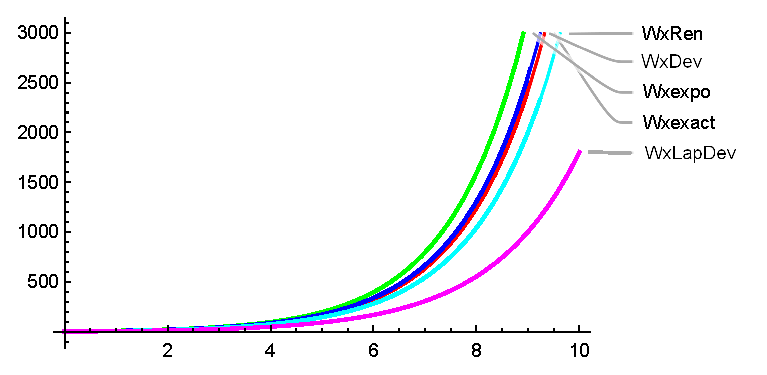
\includegraphics[width=\textwidth]{Wsample2}
        \caption{$W_q(x)$}
        \label{fig:Wsample2}
    \end{subfigure}
    ~ %add desired spacing between images, e. g. ~, \quad, \qquad, \hfill etc. 
      %(or a blank line to force the subfigure onto a new line)
    \begin{subfigure}[b]{0.4\textwidth}
        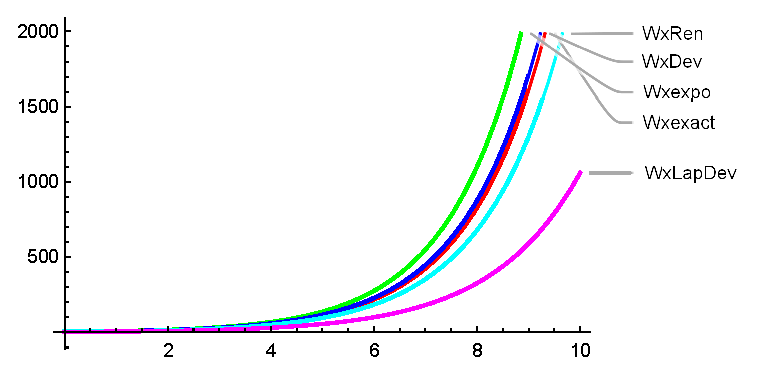
\includegraphics[width=\textwidth]{W1sample2}
        \caption{$W'_q(x)$}
        \label{fig:W1sample2}
    \end{subfigure}
    ~ %add desired spacing between images, e. g. ~, \quad, \qquad, \hfill etc. 
    %(or a blank line to force the subfigure onto a new line)
    \\
    \begin{subfigure}[b]{0.9\textwidth}
        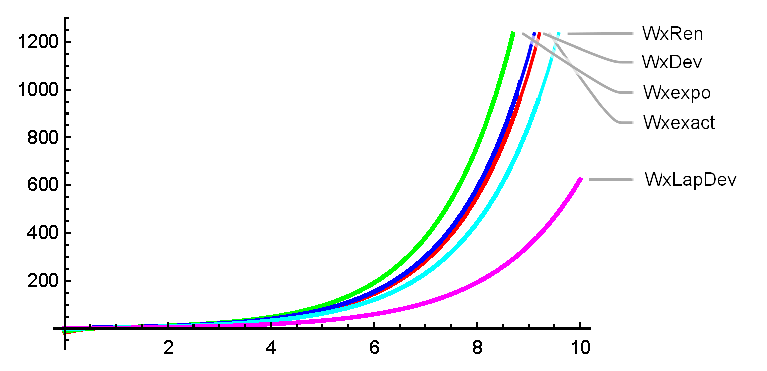
\includegraphics[width=\textwidth]{W2sample2}
        \caption{$W''_q(x)$}
        \label{fig:W2sample2}
    \end{subfigure}
    \caption{Example 2: Plots of $W_q(x)$, $W'_q(x)$, and $W''_q(x)$ of the exact solution and the approximations}\label{fig:sample2}
\end{figure}

The approximations for  $W_q(x)$ give again  Renyi and classic \deV as champions.
The dominant exponents of the Renyi and \deV s are $0.650448$, $0.670061$, one below and one above    the real $\Fq=0.666084$. This suggests that the average of the two approximations would improve on both of them.

\iffalse
\figu{W2}{}{}
\fi


    The exact optimal barrier is $b^*=0.538,$ the Renyi optimal barrier is $b_R= 0.260532$, and the relative error is $0.515739$.
    Both $W_q''$ and its \app\ are increasing \funs.

    --see \cite{johnson1989matching} for more hardest types of approximations; therein the case of mixture of Erlang distributions of sufficiently high common order was investigated.



\eeXa



\beXa

In The following example, we take a Cram\'{e}r-Lundberg process with
\bea c=\frac{7}{18},  \l=\frac{47}{60}, \th= 1\eea
and non-hyperexponential density of claims $f(x)=\frac{5}{2 }e^{-5x}+\frac{4}{5} e^{-4 x}+\frac{1}{5}e^{-3x}- \frac{1}{5}e^{-2x}+ \frac{1}{20}e^{-x}$.

The   scale function is %for the process  in Example \ref{ex1} is
  \bea
  \begin{aligned}
&  W_\q(x)  =  -0.083013\ 2.71828^{(-4.45457 x)} - 0.193651\ 2.71828^{(-3.43626 x)} -
 0.459603\ 2.71828^{(-0.855781 x)} \\
  & + 4.15668\ 2.71828^{(0.454369 x)} -  0.84898\ 2.71828^{(-2.21816 x)} \cos[0.513884 x] + 1.24626\ 2.71828^{(-2.21816 x)} \sin[0.513884 x]
\end{aligned}
  \eea

\begin{table}[]
\begin{tabular}{|l|l|l|l|l|}
\hline
       & \begin{tabular}[c]{@{}l@{}}Dominant   exponent \\ Phi\_q\end{tabular} & \begin{tabular}[c]{@{}l@{}}Percent   relative error\\ (Phi\_q)\end{tabular} & \begin{tabular}[c]{@{}l@{}}Optimal barrier\\ b*\end{tabular} & \begin{tabular}[c]{@{}l@{}}Percent   relative error\\ (b*)\end{tabular} \\ \hline
Exact  & 0.420145                                                              & 0                                                                           & 0.797999                                                     & 0                                                                       \\ \hline
Expo   & 0.429586                                                              & 2.247081365                                                                 & 0.857445                                                     & 7.449382769                                                             \\ \hline
Dev    & 0.420885                                                              & 0.17612967                                                                  & 0.0686674                                                    & 91.39505187                                                             \\ \hline
Renyi  & 0.416601                                                              & 0.843518309                                                                 & 0.794273                                                     & 0.466917878                                                             \\ \hline
LapDev & 0.392412                                                              & 6.600816385                                                                 & 0.271363                                                     & 65.99456892                                                             \\ \hline
\end{tabular}
\caption{Example 3: Values of $\Phi_q$ and $b^*$ obtained from the approximations and percent relative error when compared to the exact value}
\label{table:sample3}
\end{table}


\begin{figure}
    \centering
    \begin{subfigure}[b]{0.4\textwidth}
        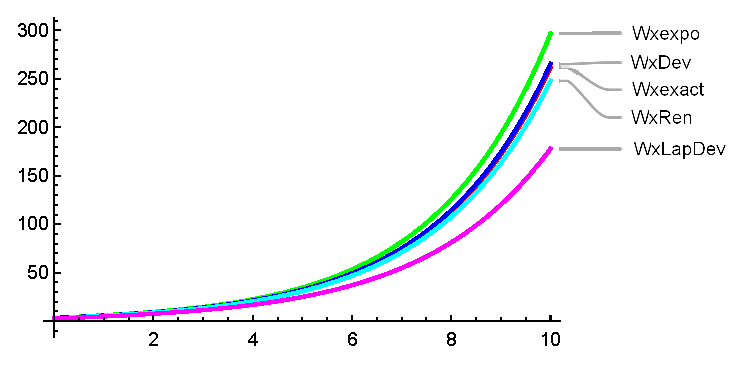
\includegraphics[width=\textwidth]{Wsample3}
        \caption{$W_q(x)$}
        \label{fig:Wsample3}
    \end{subfigure}
    ~ %add desired spacing between images, e. g. ~, \quad, \qquad, \hfill etc. 
      %(or a blank line to force the subfigure onto a new line)
    \begin{subfigure}[b]{0.4\textwidth}
        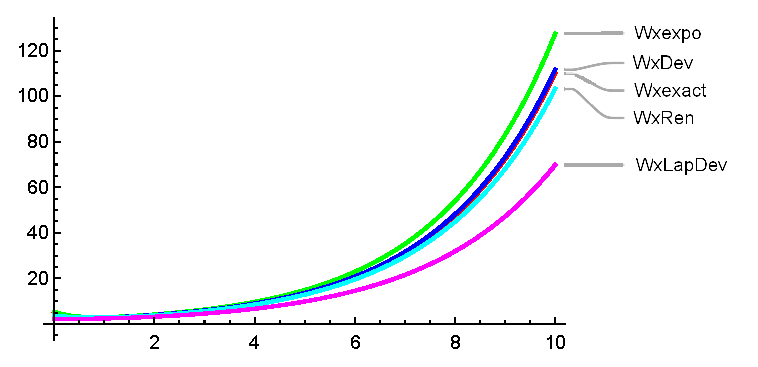
\includegraphics[width=\textwidth]{W1sample3}
        \caption{$W'_q(x)$}
        \label{fig:W1sample3}
    \end{subfigure}
    ~ %add desired spacing between images, e. g. ~, \quad, \qquad, \hfill etc. 
    %(or a blank line to force the subfigure onto a new line)
    \\
    \begin{subfigure}[b]{0.9\textwidth}
        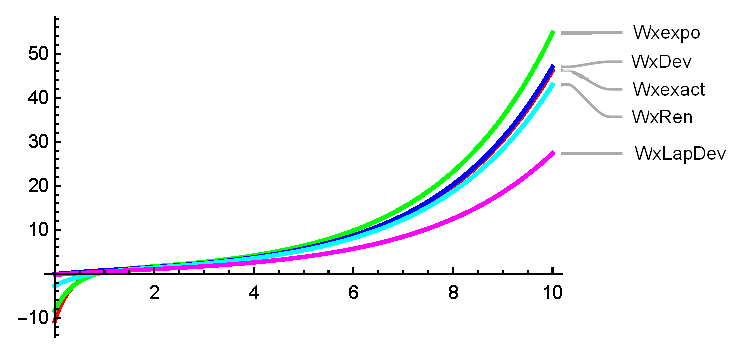
\includegraphics[width=\textwidth]{W2sample3}
        \caption{$W''_q(x)$}
        \label{fig:W2sample3}
    \end{subfigure}
    \caption{Example 3: Plots of $W_q(x)$, $W'_q(x)$, and $W''_q(x)$ of the exact solution and the approximations}\label{fig:sample1}
\end{figure}

In this case, the approximations for  $W_q(x)$ give Renyi as winner.
The dominant exponents of the Renyi and \deV s are $0.44982$, $0.455485$, one below and one above    the real $\Fq=0.454369$.
\iffalse
\figu{Wa2a}{}{}
\fi

    The exact optimal barrier is $b^*=0.779653,$ the Renyi optimal barrier is $b_R=0.732339$, and the relative error is $0.060686$.
    Both $W_q''$ and its \app\ are increasing \funs.


\eeXa



\beXa
Next we consider a more challenging example from BUTools,   produced by taking
a Cram\'{e}r-Lundberg process with matrix exponential, non phase-type  density of claims $f(x)=\a e^{A x} (-A) \bff 1, $ where $\a=(-2.4, 0.9 , 2.5),  A = \bep
   {-6.2, 2, 0}\\
   {2, -9, 1}\\
   {1, 0, -3}\eep$
and $  \th= 1, q=1/10.$

--see \cite{harris1992note} and \cite{reintelek14} for other tricky densities.


The   scale function is %for the process  in Example \ref{ex1} is
  \bea
  \begin{aligned}
& -0.0655864 e^{-9.35143 x}+0.149742 e^{-6.89805 x}-0.676982 e^{-1.26245 x}+1.3476 e^{0.142175 x}
\end{aligned}
  \eea

\iffalse
\figu{Wa3a}{}{}
\fi

 Now $\Fq=0.142175$; the dominant exponent of the classic \deV\ is very close at $ 0.142174$, and the dominant exponent of Renyi, $0.142238$, is also close.




    The exact optimal barrier is $b^*=2.61925$,   the Renyi optimal barrier is $b^*= 2.59638$, and the relative error is $0.00873044$. For classic \deV\,
    the relative error is $0.00609153$.

    However,  we may have a surprise in  examples where $b^*$ is not the unique root of $W_q''(x)$, and we may be faced with the Azcue-Muller-Loeffen phenomenon.

\iffalse    
    \figu{pl3}{When $W_q''(x)$  exhibits oscillations, exponential approximations are bound to fail in certain regions. In our example, the minimum of $W'_q$ is still unique; otherwise, one may need to resort to higher order  Pad\'e and  Laguerre  approximations. Producing examples where $W_q''(x)$   exhibits more than   three roots
and investigating the convergence of the roots of our Pad\'e approximations  seem both  hard problems.}{}
\fi
\eeXa

\iffalse
\beXa
Inspired by the density given in \cite{harris1992note}, we take in the following example a \CL \ process with
$$ \th = \frac{48}{55}, \quad \mbox{and}\ \l =1$$
with non-hyperexponential density of claims given by
$ f(x)= 3 e^{-x} - 6 e^{- 2x} +3 e^{- 3x}$
the scale function is :
 \bea \begin{aligned} & W_q (x) = -0.280452\ 2.71828^{(-0.421202 x)} + 0.540968\ 2.71828^{(0.0578629 x)} +
 0.0307461\ 2.71828^{(-2.65814 x)} \cos[0.323643 x] \\
  &+ 0.0791481\ 2.71828^{(-2.65814 x)} \sin[0.323643 x] \end{aligned} \eea

Similar to the previous example of a non-phase-type density, the approximation of $W_q$ give the classic DeVylder approximation as winner.
 \figu{wa4}{}{}

 The exact optimal barrier is  $b^*=6.9158 $,   the Renyi optimal barrier is $b_R= 6.79333$, and the relative error is $9.46103$.
 $\Phi_q = 0.0578629$; The dominant exponents of the Renyi is close at $0.0578967$ and the dominant exponent of the classic DeVylder is very close at $0.0578619.$

\figu{wsec4}{}{}

\eeXa


\beXa
We take advantage of the example presented in \cite{reintelek14}; now by taking
a Cram\'{e}r-Lundberg process with matrix exponential, non phase-type  density of claims $f(x)=\a e^{A x} (-A) \bff 1, $ where $\a=(3.99334, -5.99002, 4.32612, -1.99667, 0.667221),  A = \bep
   {-1, 1, 0, 0, 0}\\
 {0, -1, 1, 0, 0}\\
 {0, 0, -1, 1, 0}\\
 {0, 0, 0, -1, 1}\\
 {0, 0, 0, 0, -1}
\eep$ and $  \th= 1, q=1/10$.
\figu{wPH}{}{}

In this case the classic DeVylder approximation is the champion.

\figu{wPH2}{}{}

Now $\Phi_q = 0.016699$;  the dominant exponent of the classic \deV\ is very close at $ 0.0166987$, and the dominant exponent of Renyi, $0.0167116$, is also close.



 The exact optimal barrier is $b^*=21.7388 $,   the Renyi optimal barrier is $b_R= 21.7041$, and the relative error is $0.00159435 $.
\eeXa


\beXa
Another very interesting example, also inspired from \cite{reintelek14}, but this time
we take a Cram\'{e}r-Lundberg process with matrix exponential, non phase-type  density of claims $f(x)=\a e^{A x} (-A) \bff 1, $ where $\a=(1, -0.7, 0.7),  A = \bep
 {-2, 2, 0}\\
 {0, -5, 5}\\
 {0, 0, -9}
\eep$ and $  \th= 1, q=1/10$.
\figu{wPH0}{}{}
 Here the classic \deV\ approximation is also the winner.



Now $\Phi_q =0.137583 $;  the dominant exponent of the classic \deV\ is very close at $ 0.137579$, and the dominant exponent of Renyi, $0.137688$, is also close.
\figu{wPH1}{}{}



 The exact optimal barrier is $b^*=2.91429  $,   the Renyi optimal barrier is $b_R= 2.81849 $, and the relative error is $ 0.0328731  $.


 Note that the Exact $W'$ diverge from the plot of the classic Renyi, \figu{wRn}{}{}

 and so as in the plot of the Naive approximation of $W$ and the Exact $W''$. \figu{wNa}{}{}

\eeXa

\beXa
In the following example, for a Cram\'er Lundberg model we take the hyperexpoential density of claims given in \cite{avram2011moments} by  $f(x)= \frac{315}{12 }e^{-5x}+\frac{7}{8} e^{-4 x}+\frac{27}{64}e^{-3x}+ \frac{3}{16}e^{-2x}+ \frac{7}{128}e^{-x}$, with $\th = \frac{48}{55}$;


The scale function is

\bea \begin{aligned}
& W_q (x)= -0.00493814\ 2.71828^{(-4.07091 x)} - 0.0558297\ 2.71828^{(-3.19893 x)} -
 0.196449\ 2.71828^{(-2.54279 x)}\\
 & - 0.123323\ 2.71828^{(-1.83918 x) }- 0.0646808\ 2.71828^{(-0.941267 x)} + 0.87134\ 2.71828^{(0.0892008 x)} \end{aligned}\eea
\figu{wAv}{}{}

We notice again that the classic DeVylder is the winner.


And here $\Phi_q = 0.0892008$; the dominant exponent of the classic \deV\ is very close at $ 0.0892021$, and the dominant exponent of Renyi, $0.0891807$, is also close.
\figu{wAv0}{}{}


The exact optimal barrier is $b^*=2.70201 $,   the Renyi optimal barrier is $b_R= 2.74935 $, and the relative error is $0.0175198  $.


\eeXa

\fi

    \iffalse


    {\bf The Pad\'e Tijms \app \ is $b^*=0.876898$}.
    %
The input to the \LTW \ inversion is
     \[ \H G (s)=\frac{216 \left(261 s^2+1155 s+1202\right)}{187 (6 s+5) (6 s+11) (6 s+17)},\]
the  Pad\'e approximation of order $(0,1)$ is $\frac{312077664}{187 (1278399 s+1123870)}$,  the Laguerre exponent is $\alpha/2=0.879123$, and the largest error with $n=40$ is $4 \times 10^{-14}$ -- see Figure \ref{f:err3}.
\figu{err3}{Relative errors of the \LTW \ inversion with mixed exponential claims of order $3$}{}

Again, the exponent  $\alpha/2=\fr{ 6 \k'(\Fq) \k''(\Fq)}{3 (\k''(\Fq))^2- \k'(\Fq) \k'''(\Fq)}=1.138$ does better,  with the largest error  with $n=40$ of $6 \times 10^{-16}$.  This suggests the importance of optimizing $\a$, which is a  difficult problem \cite{giunta1989more,weideman1999algorithms}.  Recall however our proposal  to circumvent it by starting with a
higher order \Pd \ of $G(s)$ -- see \eqref{MG}.
 Another reasonable choice is the ``true dominant exponent  $\alpha/2=5/6$ which is unknown in real life, and yields a larger error $3 \times  10^{-15}$ (with $n=50$). The exponent of the new  formula \eqref{al} is $\alpha/2=0.77$, and the  error with $n=50$ is $3 \times 10^{-14}$, even larger.
%\fi
In  the figure \ref{f:MEp2}, we draw the exact $W_q$, together with its six   approximations.
\fi
\iffalse


 \figu{}{\label{Erl(2)} Approximations of the scale function pour sinistres Erlang(2,2), $\r=.84$ en gras pointill\'e, avec Tijms tr\`es proche dessous. L'approx. exponentielle en bas est la pire. De Vylder (pointill\'e) et Renyi sont tr\`es proches pour $u>3$, et leur moyenne fait encore mieux pour $u<3$.}
{0.7}
\fi
 \input{315}
%\input{NH5} %bad graphs
%\input{NH5bic} %bad graphs

%
\newpage

\subsection{A Cram\'{e}r-Lundberg process with matrix exponential, non phase-type  density %from \cite{reintelek14}
} \label{MatExp11000}

We recall first a result of \cite{Ocinneide97}:
\beP
 A \me\ density  $f(x)$ is \PH iff it has no zeroes   and if the matrix $A$  has a dominant real eigenvalue.\eeP

 \begin{figure}[!h]
    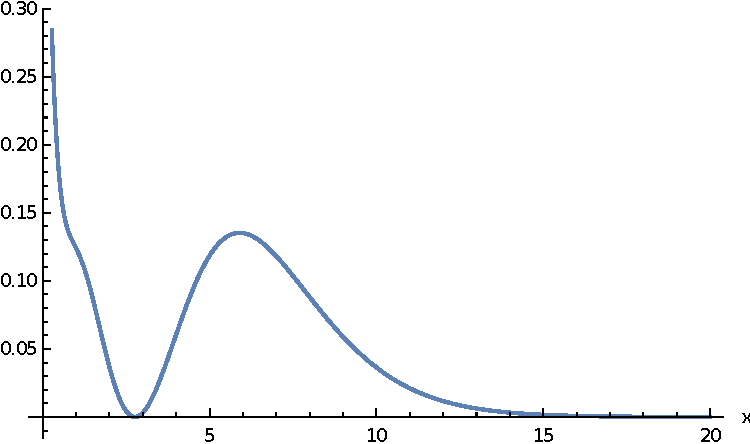
\includegraphics[width=\textwidth]{fRA1}
        \caption{A matrix-exponential density that touches the $x$ axis at $2.76434.$}
        \label{fig:fRTA1}
        \end{figure}

  We consider now a modification of a \PH example from \cite{reintelek14}, with  $f(x)=\a e^{A x} (-A) \bff 1, $ where
 \bea
   A = \bep
   {-1, 1, 0, 0, 0}\\
 {0, -1, 1, 0, 0}\\
 {0, 0, -1, 1, 0}\\
 {0, 0, 0, -1, 1}\\
 {0, 0, 0, 0, -1}
\eep \eea
and
 $$\a=(3.99334, -5.99002-\e_1, 4.32612, -1.99667-\e_2, 0.667221),$$
with $\e_1=\ 0.402289,\e_2=\ -0.402298$
 chosen so that  the resulting density touches the $x$ axis.\\
 
 The symbol of this model is given by
 \bea
\k (s)=  s \left[9.7086\, -1 \left(\frac{0.332779}{(s+1)^2}+\frac{1.92715}{(s+1)^3}-\frac{2.39897}{(s+1)^4}+\frac{3.99334}{(s+1)^5}+\frac{1}{s+1}\right)\right]
 \eea



Taking now $\th= 1,\ q=1/10$

The scale function is 
\bea
\begin{aligned}
& W_q (x)= (0.00955665\, -0.00561898 i) e^{(-1.67614+0.60724 i) x}+(0.00264501\, -0.0135933 i) e^{(-0.690461+0.703457 i) x}\\
& +(0.00955665\, +0.00561898 i) e^{(-1.67614-0.60724 i) x}+(0.00264501\, +0.0135933 i) e^{(-0.690461-0.703457 i) x}\\
& -0.103552 e^{-0.172808 x}+0.18215 e^{0.0193028 x}
\end{aligned}
\eea

\begin{figure}[!h]
\begin{subfigure}[a]{0.9\textwidth}
        \includegraphics[width=\textwidth]{wRA}
        \caption{$W_q(x)$}
        \label{fig:wRA}
    \end{subfigure}
    \begin{subfigure}[b]{0.9\textwidth}
        \includegraphics[width=\textwidth]{w1DR}
        \caption{$W'_q(x)$}
        \label{fig:w1DR}
    \end{subfigure}
    \begin{subfigure}[c]{0.9\textwidth}
        \includegraphics[width=\textwidth]{wRA2}
        \caption{$W''_q(x)$}
        \label{fig:wRA2}
    \end{subfigure}
    \caption{ Plots of $W_q(x)$, $W_q'(x)$ and $W''_q(x)$ of the exact solution and the approximations, for the \cite{reintelek14} example.}
\end{figure}




  The dominant exponent of the classic \deV\ and of Renyi are $0.0193023$,$0.0193208$; one below and one above the real $\Phi_q = 0.0193028 $.


 The exact optimal barrier is $b^*=19.8797 $,   the Renyi optimal barrier is $b_R= 19.5007$, and the relative error is $0.0190613 $.



\begin{table}[!h]
\begin{tabular}{|l|l|l|l|l|}
\hline
       & \begin{tabular}[c]{@{}l@{}}Dominant   exponent \\ $\Phi_q$\end{tabular} & \begin{tabular}[c]{@{}l@{}}Percent   relative error\\ ($\Phi_q$)\end{tabular} & \begin{tabular}[c]{@{}l@{}}Optimal barrier\\ $b^*$\end{tabular} & \begin{tabular}[c]{@{}l@{}}Percent   relative error\\ ($b^*$)\end{tabular} \\ \hline
Exact  &0,0166877                                                               & 0                                                                           & 21,7474                                                      & 0                                                                       \\ \hline
Expo   & 0,00896832                                                              & 46,25790253
 & 1,57723                                                      & 92,74750085
 \\ \hline
Dev    & 0,0166874                                                              & 0,001797731
 & 21,5985                                                      & 0,684679548
 \\ \hline
Renyi  & 0,0166959                                                             & 0,049137988
 & 21,7417                                                      & 0,02621003
 \\ \hline
LapDev &0,0128023                                                              & 23,28301683
 & 20,6235                                                      & 5,167974103                                                             \\ \hline
\end{tabular}
\caption{Values of $\Phi_q$ and $b^*$ obtained from the approximations and relative error s when compared to the exact value. }
\label{table:ReinAv}
\end{table}
The approximations for $W_q(x)$ give Renyi and the classic \deV\ as winners.

We can  see from Table \ref{table:ReinAv}, that the relative error  $(\Phi_q)$ is too small (less than $1 \%$) for both DeVylder's and Renyi's approximations, with \deV\ beating them all. Considering the values of the optimal barrier $b^*$ for all the approximations, we notice that the relative error  is the smallest (less than $1 \%$) in the case of Renyi approximation.

%\newpage 
%\subsection{A \per\ Cram\'{e}r-Lundberg process} \label{e:Loeffen}
In the following example, we study, following    \cite{Loe08}, a perturbed \CL\ model with Erlang  $Erlang(2,1)$  density of claims $f(x) = 10 \le(x \a^2 e^{-x}\ri)$ for $\a =1$, and  $\l=10,\ \th = \frac{1}{10},\  c = \frac{107}{5},\ q=\frac{1}{10}.$

The scale function when the volatility parameter is $\s =2$ is given by
\bea
\begin{aligned}
& W_q (x) =-0.0431493\ 2.71828^{-11.1486 x}+0.00613626\ 2.71828^{-1.5136 x}-0.232557\ 2.71828^{-0.0765082 x}\\
& +0.26957\ 2.71828^{0.0387284 x}
\end{aligned}
\eea

\begin{figure}[!h]
\begin{subfigure}[a]{0.9\textwidth}
        \includegraphics[width=\textwidth]{WLoefa}
        \caption{Graphs of $W_q$ in the Loeffen example with $\k(s)= \frac{\s^2 s^2}{2}+ s \left(c- \l \le(\frac{1}{(s+1)^2}+\frac{1}{s+1}\ri)\ri) , \s = 2, \ c= \frac{107}{5}$. The classic \deV \ and the Renyi approximation are indistinguishable from the exact.}
        \label{fig:WLoefa}
    \end{subfigure}
\begin{subfigure}[b]{0.9\textwidth}
        \includegraphics[width=\textwidth]{ShLoe}
        \caption{Graphs of $W_q'$ in the Loeffen example.}
        \label{fig:ShLoe}
    \end{subfigure}

    \begin{subfigure}[c]{0.9\textwidth}
        \includegraphics[width=\textwidth]{WLoefb}
        \caption{$W''_q(x)$, $\s = 2$}
        \label{fig:WLoefb}
    \end{subfigure}
    \caption{Graph of $W_q(x),W'_q(x),W''_q(x)$ and its approximations and the approximations in the Loeffen example.}
\end{figure}
\BEN
\im When $\s=2$: $\Phi_q = 0.0387284$; the dominant exponent of the classic \deV \ is very close at $0.0395652$, and the dominant exponent of Renyi, $0.0396427$, is also close.
The exact optimal barrier is $b^{*}= 10.5345$, the Renyi optimal barrier is $b_R = 10.2346$, and the relative error $0.0284683$.
 The DeVylder optimal barrier is $b_V= 10.5213$, and the relative error for the classic \deV\ is $0.00124852$.

 \im When $\s= \frac{7}{5}$: $\Phi_q = 0.0391484$; the dominant exponent of the classic \deV \ is very close at $0.0395652$, and the dominant exponent of Renyi, $0.0396427$, is also close.
The exact optimal barrier is $b^{*}= 10.4389$, the Renyi optimal barrier is $b_R = 10.1742$, and the relative error $0.0253614$.
 The DeVylder optimal barrier is $b_V= 10.4653$, and the relative error for the classic \deV\ is $0.00252756$.
 \EEN





    \iffalse


    {\bf The Pad\'e Tijms \app \ is $b^*=0.876898$}.
    %
The input to the \LTW \ inversion is
     \[ \H G (s)=\frac{216 \left(261 s^2+1155 s+1202\right)}{187 (6 s+5) (6 s+11) (6 s+17)},\]
the  Pad\'e approximation of order $(0,1)$ is $\frac{312077664}{187 (1278399 s+1123870)}$,  the Laguerre exponent is $\alpha/2=0.879123$, and the largest error with $n=40$ is $4 \times 10^{-14}$ -- see Figure \ref{f:err3}.
\figu{err3}{Relative errors of the \LTW \ inversion with mixed exponential claims of order $3$}{}

Again, the exponent  $\alpha/2=\fr{ 6 \k'(\Fq) \k''(\Fq)}{3 (\k''(\Fq))^2- \k'(\Fq) \k'''(\Fq)}=1.138$ does better,  with the largest error  with $n=40$ of $6 \times 10^{-16}$.  This suggests the importance of optimizing $\a$, which is a  difficult problem \cite{giunta1989more,weideman1999algorithms}.  Recall however our proposal  to circumvent it by starting with a
higher order \Pd \ of $G(s)$ -- see \eqref{MG}.
 Another reasonable choice is the ``true dominant exponent  $\alpha/2=5/6$ which is unknown in real life, and yields a larger error $3 \times  10^{-15}$ (with $n=50$). The exponent of the new  formula \eqref{al} is $\alpha/2=0.77$, and the  error with $n=50$ is $3 \times 10^{-14}$, even larger.
%\fi
In  the figure \ref{f:MEp2}, we draw the exact $W_q$, together with its six   approximations.
\fi
\iffalse


 \figu{}{\label{Erl(2)} Approximations of the scale function pour sinistres Erlang(2,2), $\r=.84$ en gras pointill\'e, avec Tijms tr\`es proche dessous. L'approx. exponentielle en bas est la pire. De Vylder (pointill\'e) et Renyi sont tr\`es proches pour $u>3$, et leur moyenne fait encore mieux pour $u<3$.}
{0.7}
\fi

\newpage 
%\input{RTnon}

%\input{mod}
\section{Optimizing dividends and \ci \cite{Gaj,AGLW} \la{s:AG}}
We refer to \cite{Gaj,AGLW}  for the formulation of this stochastic control problem.

 In this section we revisit the   problem of optimizing numerically the value of "bounded buffer $(-a,0,b)$ policies", which
consist in allowing capital injections smaller than a given $a$ and declaring bankruptcy at the first time when the size of the overshoot below 0 exceeds $a,$ and  pay dividends when the reserve reaches an upper barrier $b$.
\subsection{The cost function and its optimization \la{s:cost}}
We  present here a synthesis of the  results of \cite{Gaj,AGLW} (in order  to relate the results, one needs to replace  $\g$ in the  objective of \cite{Gaj} by  $1/k$).  They are
expressed  in terms of the functions
\be \la{RG} \bc R_a(x) =\l \int_0^x W_q(x-y) \;   \ovl F(y+a)  \; dy \\G_a(x)=\l \int_0^x  W_q(x-y) \;  m_y(a) \; \; dy, \; \; \; \; m_y(a)=\int_0^a z f(y+z)dz\\S_a(x)=Z_q(x)+  R_a(x)\ec \ee
(\cite{Gaj} use $s_c,r_c$, instead of $G_a(x),R_a(x)$, \resp).

\beR The relation \eqr{J0} below earns the function $S(x,a)$ the name of scale function for our problem, which basically means that it will appear in several different problems involving a reflecting barrier at $b$ and a limited reflection buffer $(-a,0]$. See \cite[Rem. 8]{AGLW} for some other examples, and see the equation \cite[(3)]{Gaj} for an additional example. \eeR

\beR \la{r:idG} Cf. \cite[Lem. A.4]{Gaj}, these functions \saty
\be \la{idG} G_a(x)+a R_a(x)=\int_0^a R_y(x)dy =\l \int_0^x W_q(x-y) \int_0^a \ovl F(y+z) dz dy \Lra \bc  G_{a'}(x)= -a  R_{a'}(x)\\G_a'(x)+a R_a'(x)= \int_0^a R_y'(x)dy \ec,\ee
where
 $R_{a'}(x),G_{a'}(x)$ denote derivatives with respect to the subscript, and
where we added a missing minus in the last statement of \cite[Lem. A.4]{Gaj}.
\eeR
\beXa
In the particular case of \expoj, the functions \eqr{RG}  become \cite{AGLW}
$$\bc G_a(x)=  C_\q(x) m(a), \; R_a(x)=
C_\q(x)e^{- \mu  a}, \\ C_q(x)=c W_q(x)- Z_q(x), \; m(a)=\int_0^a y \; F( \md y)=\frac{1-e^{-\mu a } (\mu a +1)}{\mu }\ec,$$
as follows
from the identities $\ovl F(y+a)=e^{-\mu a} \ovl F(y), m_y(a)= e^{-\mu y} m(a)$.

Note also the formulas \be \la{heur} \bc
R_a(x) =  C_\q(x) (1-F(a))\\  G_a(x)=
C_\q(x) \int_0^a y \; F( \md y) %{+k \si W_q(x), \text{ cf sols 2,3?}}
\ec, \ee
which will be used below as a heuristic approximation in non-\expo\ cases.

\eeXa

\beXa

Consider now the more general case when the claims are distributed according to a matrix exponential density generated by a row vector $\vb$ and by an invertible matrix $B$ of order $n$, which are such that the vector $\vb e^{ x B}$ is decreasing componentwise to $0$, and $\vb . \vo \neq 0 $, with $\vo %, \bff b
$ a  column vector. As customary, we  restrict \wlo to the case
when  $\vb$ is a probability vector, and  $\vb . \bff 1 =1$, so that  $$\ovl F(x)=%(\vb . \vo)^{-1}
\vb e^{ x B} \vo$$  is a valid survival function.


 The matrix versions of our  functions are:

  \be \la{mpf} \bc R_a(x) =\l \int_0^x W_q(x-y) \;   \ovl F(y+a)  \; dy = \l \vb \int_0^x W_q(x-y) \;e^{ y B}     \; dy  \; e^{ a B} \vo= \vec C_q(x) e^{ a B} \vo
 \\ m_y(a)=\int_0^a z f(y+z)dz=\vb  \; e^{ y B} \; \int_0^a z \;e^{ z B} (-B)    \; dz \;\vo=\vb   \; e^{ y B} M(a) \vo
 \\G_a(x)=\l \int_0^x  W_q(x-y) \;  m_y(a) \; \; dy= \vec C_q(x) M(a) \vo \; \; \; \; \ec, \ee
 where
\be \bc C_q(x)=\l  \int_0^x W_q(x-y) \;e^{ y B}     \; dy\\
\vec C_q(x)=\l \vb \int_0^x W_q(x-y) \;e^{ y B}     \; dy \ec. \ee

The product  formulas \eqr{mpf} may also be established directly in the \PH case,  using the conditional independence of the ruin probability of the overshoot size -see section \ref{s:me}.
\eeXa

\beP \cite[Thm. 4]{Gaj} {\bf Cost function  for $(a,b)$ policies} \la{l:intfper}

 For a % {\per}
\CL process  (\cP) with \expoj, let
$$J_x=J^{a,b}(x):=
\mathbb{E}_x\pp{\int_0^{\ta}e^{-qt}\pr{\md \D_t -k \;\md\C_t}}  $$
denote the \eddc\ associated to policies consisting in paying capital injections  with proportional cost $k\geq 1$, provided that the severity of ruin is smaller than $a>0$, and paying dividends as soon as the  process reaches some upper level $b$.


 Then,\BEN \im
 \be J_x= \bc k G_a(x) +J_0^{(a,b)} S_a(x)=k G_a(x) +\fr{1-k G_a'(b)}{S_a'(b)} S_a(x),  &x \in[0, b]\\k x+J_0^{(a,b)}
&x \in[-a, 0]\\ 0 & x \leq -a \ec. \la{struct}\ee
\im  For fixed  $b\geq 0$, the optimality equation $\fr{\partial}{\partial a} J_0^{a,b}=0$  \mbw \be \la{paa}
 k a= J_0^{a,b} \Eq J_{-a}^{a,b}= 0. \ee

\EEN
\eeP
\prf The first statement is \cite[Thm. 4]{Gaj}, and the second is a consequence of \eqr{idG}.\qed

In the \expo\ case, further simplification is possible. In particular, we will take advantage of properties of the Lambert-W function, which were not exploited in \cite{AGLW}.
\beC {\bf Cost function and  optimality conditions in the \expo\ case}
\BEN \im
  \be J_0^{(a,b)}=
\fr{1-k \; m(a) C_\q'(b)}{(1-F(a)) C_\q'(b) + q W_q(b)}=\frac{{\g(b)}-k \;  m(a) }
{ 1-F(a)+q \th(b)}, \la{J0}
 \ee
where we put $$ \g(b)=\fr{1}{C_q'(b)}, \th(b)=\fr{W_q(b)}{C_\q'(b)}.$$

 \im For fixed  $a\geq 0$, the optimality equation $\fr{\partial}{\partial b} J_0^{a,b}=0$  \mbw

\be  J_0^{a,b}  =j(b), \; j(b):= \fr{ \g'(b)}{q  \th'(b)}. \la{jb}\ee

At a critical point $(a^*,b^*), a^*>0, b^* >0$,  \wmh\ $J_0^{a^*,b^*}  =j(b^*)=k a^* \Lra$
\be    a^* =s(b^*), s(b):=\fr{j(b)}k. \la{J0a}\ee

In conclusion, $b^*$ for such critical points may be computed solving
\be \la{str} %q \th(b) j(b)+ \fr k{\mu} \pr{1- e^{-\mu a}}=\g(b) \Eq
 \eta(b):=\fr{\g(b)}{\th(b)}-q  j(b) - \fr k{\mu \th(b)}  F\pr{\fr{j(b) }{k}}=0. \ee


\beR  a) The important equation \eqr{J0a} identifies  the optimal buffer associated with a dividends barrier $b$ via the explicit function $s(b)$. In the general framework of \cite{Gaj}, $s(b)$ is only defined implicitly as solution of   \cite[(6)]{Gaj}.

b) For fixed  $b\geq 0$, the optimality equation $$\fr{\partial}{\partial a} J_0^{a,b}=0  \Eq  J_0^{(a,b)}= k a  =
 {
 \fr{\g(b)- k m(a)}
 {e^{-\mu a}+ q\th(b)}}$$
 \mbw also as
 $k a=\fr{\g(b)- k \fr{1- e^{-\mu a}}\mu}{q\th(b)}.$

\eeR



\im  In the special case $b^*=0$, the optimality equation \eqref{paa} implies that $a^*=a_k:=a_{k,0}$ satisfies
the simpler equation
\begin{align}\label{StructureEqa}
\d(k,a):=c -k\pr{a q + \fr{\l}{\mu} F( a)  }=0. % \; c =c +
\end{align}

\EEN






 Rewriting the equation \eqr{StructureEqa} as $z e^z =\fr \l q e^{ g}, z=\mu a +g$) implies that the solution  is
$$\mu a =-g + L_W\pr{\fr \l q e^{ g}}, g=\fr{\l }{ q}-\fr{\mu c}{k q},$$
where $L_W$ denotes the real Lambert-W function \cite{corless1996lambertw,boyd1998global,brito2008euler,vazquez2019psem}
    (this observation is missing in \cite{AGLW}).
\eeC

\prf 2. From \eqr{J0}, the optimality equation $\fr{\partial}{\partial b} J_0^{a,b}
=0$ simplifies to
$$J_0^{(a,b)}=\frac{{\g'(b)} }
{ q \th'(b)}=j(b)(=-\fr{C_\q''(b)}{q\pr{ W_q'(b) C_\q'(b)-C_\q''(b)  W_q(b)}}), $$ and recalling $J_0^{(a,b)}=k a$ yields the result.
\qed

\beR Without switching to $\g, \th$, the previous computation is
more complicated
\bea J_0^{(a,b)}=
\fr{-k \; m(a) C_\q''(b)}{(1-F(a)) C_\q''(b) + q W_q'(b)}\eea

\eeR


%\iffalse
We have now a further look at  the functions introduced in Proposition \ref{l:intfper}.
\Itm $\g$ is increasing-decreasing (from $\fr c \l$ to $0$), with a maximum at
the root of $C_q''(x)=0$, which is
\be \la{bb}\bar{b}:=\frac{1}{\Phi_q-\rho_-}\log\pr{\frac{\rho_-^2}{\Phi_q^2}},\ee and $\th$ increases from %$0$ to $1/\Fq$.
%(and hence $\th$ increases from
$\th(0)=\fr{1/c}{\l/c}=\fr 1{\l}$ to $\th(\I)=\fr 1{c \Fq - q }$.%=\fr{\mu \Fq+1}{\l}$ .

The following result is to be found, albeit with somewhat different notations, in \cite[Proof of Theorem 11, A2]{AGLW}.


\beL
The function $j(b)=\frac{\g'(b)}{q \th'(b)}$ is decreasing, with  $j(0)=\fr{\l}{\mu q}\fr{-C_\q''(0)}{(C_\q'(0))^2}=
\fr{c \mu -  \pr{q +\l}}{\mu q}$. If  $c \mu -  \pr{q +\l} >0$, then $\bar{b}>0$ defined in \eqr{bb} is the unique positive root  of $j({b}) $.
\eeL



\beR Introducing
$$\eta(b,a):=\fr {\g(b)}{\th(b)} -k \pr{ q a+ \fr 1{\mu \th(b)} F\pr{a}}=\fr {1}{W_q(b)} -k \pr{ q a+ \fr 1{\mu \th(b)} F\pr{a}},$$ we note  by using $C_q'(0)=\fr \l c, W_q(0)=\fr 1 c$ that $$\eta(0,a):=c -k \pr{ q a+ \fr {\l} {\mu }  F\pr{a}}=\d(k,a).$$

The continuous function $\pp{0,\bar{b}}\ni b\mapsto\eta(b),$
\be \la{et0} \eta(b):=\eta(b,s(b))=\fr {1}{W_q(b)}   -
  q j(b) -\fr {k} {\mu \th(b)}  F\pr{s(b)}, \; s(b):=\fr{j(b) }k,\ee
  already defined in \eqr{str},
  will play an important role below.

   Note that \bea && \eta(0)=\fr c \l- \fr 1 \l \pr{c - \fr {q +\l}\mu}-\fr {k}\mu F\pr{\frac{j(0)}{k }}=\fr {1}{\l \mu} \pr{\l+  {q}-\l {k} F\pr{\frac{j(0)}{k }}}=\fr {1}{\l }\delta(k)<0.%, \forall k>k^*,
\eea

 and    $\eta\pr{\bar{b}} =\fr{1}{W_q\pr{\bar{b}}}>0$. \Thr $\eta(b)=0$  has at least one solution of in $[0,\bar{b}]$; the first such solution will be denoted by $b^*$.

 % Note that the function $s(b)$, which figures also in \cite[(6)]{Gaj}  as $c(x)$, is explicit in our setup.
\eeR

\beR Putting $h=\fr {1}{q \th(b)}-\fr {\mu } k \fr {\g(b)}{q \th(b)} ,$ the structure equation \eqr{str} may be rewritten as:
\bea (\fr {\mu } k j(b)+ h) e^{\fr {\mu } k j(b)+ h}=\fr {e^{h }}{q \th(b)}  \Lra \fr {\mu } k j(b)+h = L_w(\fr {e^{h }}{q \th(b)} ).\eea
%\be     \eta(b):=\fr {1}{W_q(b)}\pr{1 - k\fr {C_q'(b)}{\mu } F\pr{s(b)}}   -k  q s(b)+ =0. \la{str}\ee
\eeR

The following (new!) result relates the
dichotomy domains  to the  Lambert-W function.

\beL
The  function \be \d(k):=\d(k,j(0)/k)=\d(k,\fr{c \mu -  \pr{q +\l}}{k \mu q})=\mu^{-1}
\pr{\lambda+q-\lambda k\pr{1-e^{-\frac{c\mu-\lambda-q}{qk}}}}
\ee
has a unique  \nne\ root
$k^*$  iff
\begin{equation}
\label{Cheapk}c \mu>\lambda^{-1} \pr{\lambda+q}^2>\pr{\lambda+q }.\end{equation}
%and $P > P_0$.,

Explicitly,
\be \la{ks} k^*=\fr{q + \l} \l \fr{f}{f + L_W\pr{- f e^{-f}}}, \; f =\fr{ \l}{q+\l} \fr{c\mu-\pr{\lambda+
q }}q. \ee




\eeL
\prf  The equation to be solved is similar to \eqr{StructureEqa}, but this time the unknown is $k$.

Putting $d =\fr{c\mu-\pr{\lambda+
q }}q $ %and $z=\frac{ d}{k}$,
 reduces the equation $\d(k)=0$ to
\bea k e^{-\frac{d}{k}}=  k-\fr{q+\l}\lambda  \Eq  e^{-\frac{d}{k}}=  1 -\fr{q+\l}{\l k} \Eq 1= e^{\frac{d}{k}}
\pr {1 -\fr{(q+\l)d}{d \l k}}:=e^{z} \pr {1 -z/f}, f=\fr{d \l}{q+\l}.
\eea

Rewriting the latter as $-f=e^{z} \pr {z -f}$  we recognize, by putting $z=y+f$,  an equation
reducible   to $ y e^{y} =- f e^{-f}, $ whose  real solution is $$y =L_W\pr{- f e^{-f}},$$ where $L_W$ denotes the real Lambert-W function. The final solution
is \eqr{ks}.

%\input{extPH}
%\input{Eq}
%\input{exaCInj}

%\input{proprei}

%\input{derDev}
%\input{nme}
\small
\bibliographystyle{amsalpha}
%\bibliographystyle{plain}
\bibliography{Pare37}
%\input{MA}
\end{document}



